%&latex
% Copyright 2011 Ruslan Kiyanchuk (c) <ruslan.kiyanchuk@gmail.com>
% 

\chapter{LINEAR TRANSFORMATION IMPACT ON KEYSTREAM PROPERTIES OF ZUC STREAM CIPHER}
\label{sec:zuc}

ZUC is a perspective stream cipher considered for use in the evolving LTE standard
for mobile communications. Its development has been handed over to Data Assurance and
Communication Security Research Center of Chinese Academy of Sciences in order
for Chinese authorities to permit its use in the country~\cite{3gpp:eea3_doc4}.

\section{Description of ZUC}


The cipher consists of three layers: linear feedback shift register (LFSR), bit
reorganization (BR) and non-linear function $F$ implemented via the finite state
machine (figure~\ref{fig:zuc})~\cite{3gpp:eea3_doc2}.
\begin{figure}[htbp]
    \centering
    % Graphic for TeX using PGF
% Title: /home/zoresvit/Documents/research/diploma/graphics/zuc.dia
% Creator: Dia v0.97.1
% CreationDate: Fri Nov 11 01:43:40 2011
% For: zoresvit
% \usepackage{tikz}
% The following commands are not supported in PSTricks at present
% We define them conditionally, so when they are implemented,
% this pgf file will use them.
\ifx\du\undefined
  \newlength{\du}
\fi
\setlength{\du}{12\unitlength}
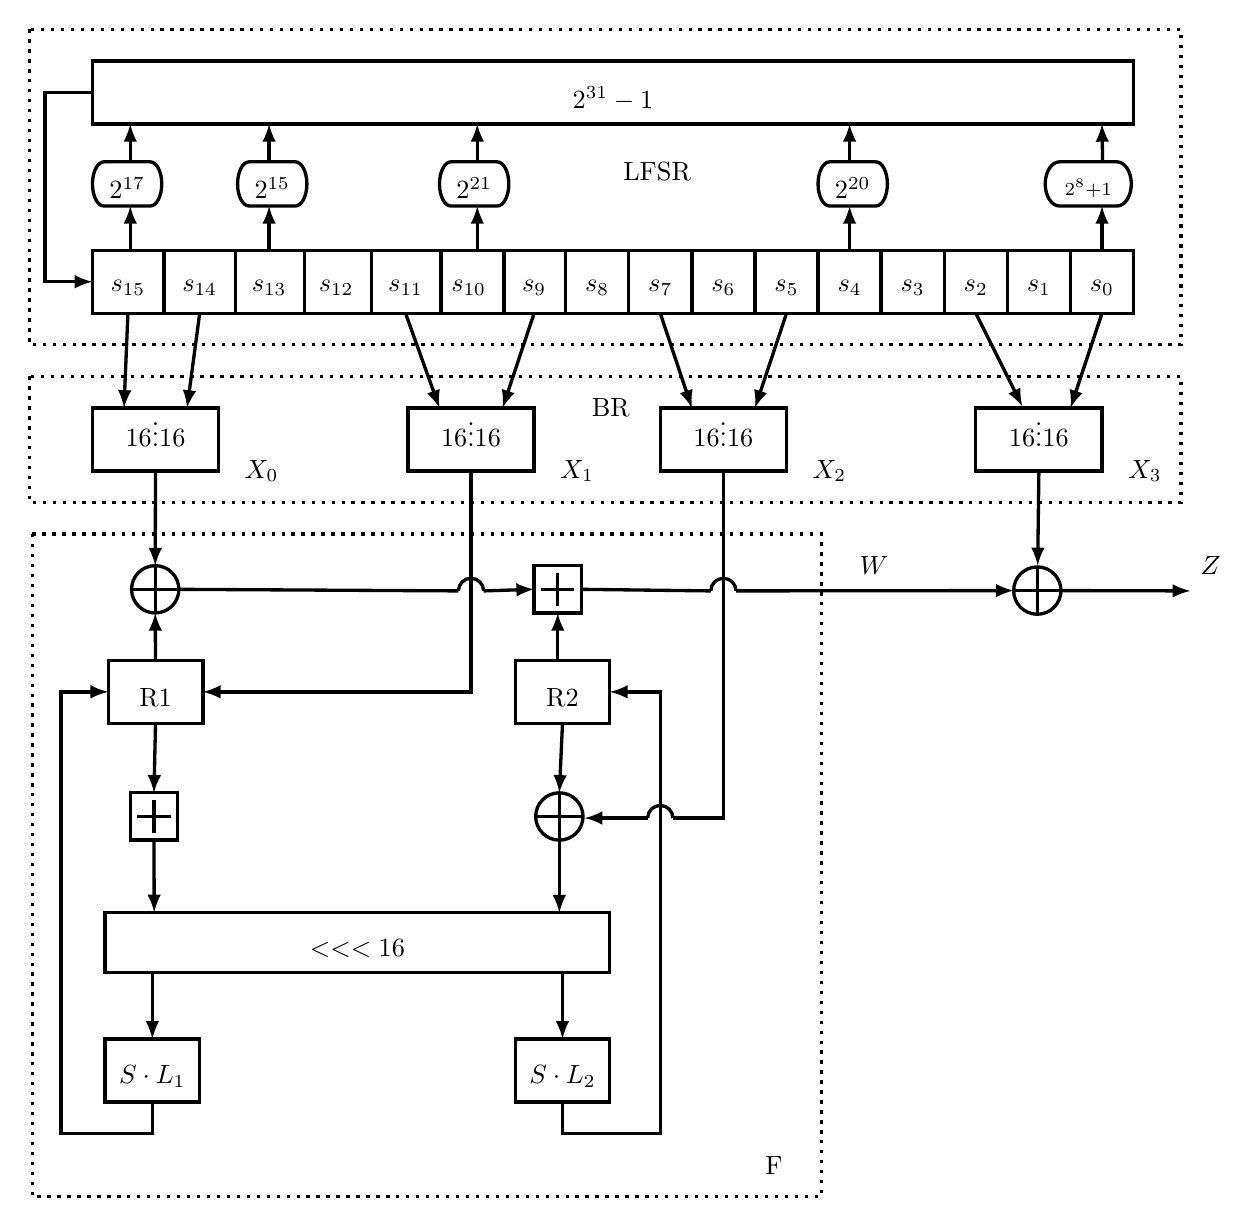
\begin{tikzpicture}[scale=0.95,every node/.style={scale=0.95}]
\pgftransformxscale{1.000000}
\pgftransformyscale{-1.000000}
\definecolor{dialinecolor}{rgb}{0.000000, 0.000000, 0.000000}
\pgfsetstrokecolor{dialinecolor}
\definecolor{dialinecolor}{rgb}{1.000000, 1.000000, 1.000000}
\pgfsetfillcolor{dialinecolor}
\pgfsetlinewidth{0.100000\du}
\pgfsetdash{{\pgflinewidth}{0.200000\du}}{0cm}
\pgfsetdash{{\pgflinewidth}{0.200000\du}}{0cm}
\pgfsetmiterjoin
\definecolor{dialinecolor}{rgb}{0.000000, 0.000000, 0.000000}
\pgfsetstrokecolor{dialinecolor}
\draw (7.000000\du,-3.000000\du)--(7.000000\du,7.000000\du)--(43.500000\du,7.000000\du)--(43.500000\du,-3.000000\du)--cycle;
% setfont left to latex
\definecolor{dialinecolor}{rgb}{0.000000, 0.000000, 0.000000}
\pgfsetstrokecolor{dialinecolor}
\node at (25.250000\du,2.195000\du){};
\pgfsetlinewidth{0.100000\du}
\pgfsetdash{{\pgflinewidth}{0.200000\du}}{0cm}
\pgfsetdash{{\pgflinewidth}{0.200000\du}}{0cm}
\pgfsetmiterjoin
\definecolor{dialinecolor}{rgb}{0.000000, 0.000000, 0.000000}
\pgfsetstrokecolor{dialinecolor}
\draw (7.000000\du,8.000000\du)--(7.000000\du,12.000000\du)--(43.500000\du,12.000000\du)--(43.500000\du,8.000000\du)--cycle;
% setfont left to latex
\definecolor{dialinecolor}{rgb}{0.000000, 0.000000, 0.000000}
\pgfsetstrokecolor{dialinecolor}
\node at (25.250000\du,10.195000\du){};
\pgfsetlinewidth{0.100000\du}
\pgfsetdash{{\pgflinewidth}{0.200000\du}}{0cm}
\pgfsetdash{{\pgflinewidth}{0.200000\du}}{0cm}
\pgfsetmiterjoin
\definecolor{dialinecolor}{rgb}{0.000000, 0.000000, 0.000000}
\pgfsetstrokecolor{dialinecolor}
\draw (7.100000\du,13.000000\du)--(7.100000\du,34.000000\du)--(32.100000\du,34.000000\du)--(32.100000\du,13.000000\du)--cycle;
% setfont left to latex
\definecolor{dialinecolor}{rgb}{0.000000, 0.000000, 0.000000}
\pgfsetstrokecolor{dialinecolor}
\node at (19.600000\du,23.695000\du){};
% setfont left to latex
\definecolor{dialinecolor}{rgb}{0.000000, 0.000000, 0.000000}
\pgfsetstrokecolor{dialinecolor}
\node[anchor=west] at (25.500000\du,1.500000\du){LFSR};
% setfont left to latex
\definecolor{dialinecolor}{rgb}{0.000000, 0.000000, 0.000000}
\pgfsetstrokecolor{dialinecolor}
\node[anchor=west] at (24.500000\du,9.000000\du){BR};
\definecolor{dialinecolor}{rgb}{1.000000, 1.000000, 1.000000}
\pgfsetfillcolor{dialinecolor}
\fill (40.000000\du,4.000000\du)--(40.000000\du,6.000000\du)--(42.000000\du,6.000000\du)--(42.000000\du,4.000000\du)--cycle;
\pgfsetlinewidth{0.100000\du}
\pgfsetdash{}{0pt}
\pgfsetdash{}{0pt}
\pgfsetmiterjoin
\definecolor{dialinecolor}{rgb}{0.000000, 0.000000, 0.000000}
\pgfsetstrokecolor{dialinecolor}
\draw (40.000000\du,4.000000\du)--(40.000000\du,6.000000\du)--(42.000000\du,6.000000\du)--(42.000000\du,4.000000\du)--cycle;
% setfont left to latex
\definecolor{dialinecolor}{rgb}{0.000000, 0.000000, 0.000000}
\pgfsetstrokecolor{dialinecolor}
\node at (41.000000\du,5.195000\du){$s_{0}$};
\definecolor{dialinecolor}{rgb}{1.000000, 1.000000, 1.000000}
\pgfsetfillcolor{dialinecolor}
\fill (38.000000\du,4.000000\du)--(38.000000\du,6.000000\du)--(40.000000\du,6.000000\du)--(40.000000\du,4.000000\du)--cycle;
\pgfsetlinewidth{0.100000\du}
\pgfsetdash{}{0pt}
\pgfsetdash{}{0pt}
\pgfsetmiterjoin
\definecolor{dialinecolor}{rgb}{0.000000, 0.000000, 0.000000}
\pgfsetstrokecolor{dialinecolor}
\draw (38.000000\du,4.000000\du)--(38.000000\du,6.000000\du)--(40.000000\du,6.000000\du)--(40.000000\du,4.000000\du)--cycle;
% setfont left to latex
\definecolor{dialinecolor}{rgb}{0.000000, 0.000000, 0.000000}
\pgfsetstrokecolor{dialinecolor}
\node at (39.000000\du,5.195000\du){$s_{1}$};
\definecolor{dialinecolor}{rgb}{1.000000, 1.000000, 1.000000}
\pgfsetfillcolor{dialinecolor}
\fill (36.000000\du,4.000000\du)--(36.000000\du,6.000000\du)--(38.000000\du,6.000000\du)--(38.000000\du,4.000000\du)--cycle;
\pgfsetlinewidth{0.100000\du}
\pgfsetdash{}{0pt}
\pgfsetdash{}{0pt}
\pgfsetmiterjoin
\definecolor{dialinecolor}{rgb}{0.000000, 0.000000, 0.000000}
\pgfsetstrokecolor{dialinecolor}
\draw (36.000000\du,4.000000\du)--(36.000000\du,6.000000\du)--(38.000000\du,6.000000\du)--(38.000000\du,4.000000\du)--cycle;
% setfont left to latex
\definecolor{dialinecolor}{rgb}{0.000000, 0.000000, 0.000000}
\pgfsetstrokecolor{dialinecolor}
\node at (37.000000\du,5.195000\du){$s_{2}$};
\definecolor{dialinecolor}{rgb}{1.000000, 1.000000, 1.000000}
\pgfsetfillcolor{dialinecolor}
\fill (34.000000\du,4.000000\du)--(34.000000\du,6.000000\du)--(36.000000\du,6.000000\du)--(36.000000\du,4.000000\du)--cycle;
\pgfsetlinewidth{0.100000\du}
\pgfsetdash{}{0pt}
\pgfsetdash{}{0pt}
\pgfsetmiterjoin
\definecolor{dialinecolor}{rgb}{0.000000, 0.000000, 0.000000}
\pgfsetstrokecolor{dialinecolor}
\draw (34.000000\du,4.000000\du)--(34.000000\du,6.000000\du)--(36.000000\du,6.000000\du)--(36.000000\du,4.000000\du)--cycle;
% setfont left to latex
\definecolor{dialinecolor}{rgb}{0.000000, 0.000000, 0.000000}
\pgfsetstrokecolor{dialinecolor}
\node at (35.000000\du,5.195000\du){$s_{3}$};
\definecolor{dialinecolor}{rgb}{1.000000, 1.000000, 1.000000}
\pgfsetfillcolor{dialinecolor}
\fill (32.000000\du,4.000000\du)--(32.000000\du,6.000000\du)--(34.000000\du,6.000000\du)--(34.000000\du,4.000000\du)--cycle;
\pgfsetlinewidth{0.100000\du}
\pgfsetdash{}{0pt}
\pgfsetdash{}{0pt}
\pgfsetmiterjoin
\definecolor{dialinecolor}{rgb}{0.000000, 0.000000, 0.000000}
\pgfsetstrokecolor{dialinecolor}
\draw (32.000000\du,4.000000\du)--(32.000000\du,6.000000\du)--(34.000000\du,6.000000\du)--(34.000000\du,4.000000\du)--cycle;
% setfont left to latex
\definecolor{dialinecolor}{rgb}{0.000000, 0.000000, 0.000000}
\pgfsetstrokecolor{dialinecolor}
\node at (33.000000\du,5.195000\du){$s_{4}$};
\definecolor{dialinecolor}{rgb}{1.000000, 1.000000, 1.000000}
\pgfsetfillcolor{dialinecolor}
\fill (30.000000\du,4.000000\du)--(30.000000\du,6.000000\du)--(32.000000\du,6.000000\du)--(32.000000\du,4.000000\du)--cycle;
\pgfsetlinewidth{0.100000\du}
\pgfsetdash{}{0pt}
\pgfsetdash{}{0pt}
\pgfsetmiterjoin
\definecolor{dialinecolor}{rgb}{0.000000, 0.000000, 0.000000}
\pgfsetstrokecolor{dialinecolor}
\draw (30.000000\du,4.000000\du)--(30.000000\du,6.000000\du)--(32.000000\du,6.000000\du)--(32.000000\du,4.000000\du)--cycle;
% setfont left to latex
\definecolor{dialinecolor}{rgb}{0.000000, 0.000000, 0.000000}
\pgfsetstrokecolor{dialinecolor}
\node at (31.000000\du,5.195000\du){$s_{5}$};
\definecolor{dialinecolor}{rgb}{1.000000, 1.000000, 1.000000}
\pgfsetfillcolor{dialinecolor}
\fill (28.000000\du,4.000000\du)--(28.000000\du,6.000000\du)--(30.000000\du,6.000000\du)--(30.000000\du,4.000000\du)--cycle;
\pgfsetlinewidth{0.100000\du}
\pgfsetdash{}{0pt}
\pgfsetdash{}{0pt}
\pgfsetmiterjoin
\definecolor{dialinecolor}{rgb}{0.000000, 0.000000, 0.000000}
\pgfsetstrokecolor{dialinecolor}
\draw (28.000000\du,4.000000\du)--(28.000000\du,6.000000\du)--(30.000000\du,6.000000\du)--(30.000000\du,4.000000\du)--cycle;
% setfont left to latex
\definecolor{dialinecolor}{rgb}{0.000000, 0.000000, 0.000000}
\pgfsetstrokecolor{dialinecolor}
\node at (29.000000\du,5.195000\du){$s_{6}$};
\definecolor{dialinecolor}{rgb}{1.000000, 1.000000, 1.000000}
\pgfsetfillcolor{dialinecolor}
\fill (26.000000\du,4.000000\du)--(26.000000\du,6.000000\du)--(28.000000\du,6.000000\du)--(28.000000\du,4.000000\du)--cycle;
\pgfsetlinewidth{0.100000\du}
\pgfsetdash{}{0pt}
\pgfsetdash{}{0pt}
\pgfsetmiterjoin
\definecolor{dialinecolor}{rgb}{0.000000, 0.000000, 0.000000}
\pgfsetstrokecolor{dialinecolor}
\draw (26.000000\du,4.000000\du)--(26.000000\du,6.000000\du)--(28.000000\du,6.000000\du)--(28.000000\du,4.000000\du)--cycle;
% setfont left to latex
\definecolor{dialinecolor}{rgb}{0.000000, 0.000000, 0.000000}
\pgfsetstrokecolor{dialinecolor}
\node at (27.000000\du,5.195000\du){$s_{7}$};
\definecolor{dialinecolor}{rgb}{1.000000, 1.000000, 1.000000}
\pgfsetfillcolor{dialinecolor}
\fill (24.000000\du,4.000000\du)--(24.000000\du,6.000000\du)--(26.000000\du,6.000000\du)--(26.000000\du,4.000000\du)--cycle;
\pgfsetlinewidth{0.100000\du}
\pgfsetdash{}{0pt}
\pgfsetdash{}{0pt}
\pgfsetmiterjoin
\definecolor{dialinecolor}{rgb}{0.000000, 0.000000, 0.000000}
\pgfsetstrokecolor{dialinecolor}
\draw (24.000000\du,4.000000\du)--(24.000000\du,6.000000\du)--(26.000000\du,6.000000\du)--(26.000000\du,4.000000\du)--cycle;
% setfont left to latex
\definecolor{dialinecolor}{rgb}{0.000000, 0.000000, 0.000000}
\pgfsetstrokecolor{dialinecolor}
\node at (25.000000\du,5.195000\du){$s_{8}$};
\definecolor{dialinecolor}{rgb}{1.000000, 1.000000, 1.000000}
\pgfsetfillcolor{dialinecolor}
\fill (22.000000\du,4.000000\du)--(22.000000\du,6.000000\du)--(24.000000\du,6.000000\du)--(24.000000\du,4.000000\du)--cycle;
\pgfsetlinewidth{0.100000\du}
\pgfsetdash{}{0pt}
\pgfsetdash{}{0pt}
\pgfsetmiterjoin
\definecolor{dialinecolor}{rgb}{0.000000, 0.000000, 0.000000}
\pgfsetstrokecolor{dialinecolor}
\draw (22.000000\du,4.000000\du)--(22.000000\du,6.000000\du)--(24.000000\du,6.000000\du)--(24.000000\du,4.000000\du)--cycle;
% setfont left to latex
\definecolor{dialinecolor}{rgb}{0.000000, 0.000000, 0.000000}
\pgfsetstrokecolor{dialinecolor}
\node at (23.000000\du,5.195000\du){$s_{9}$};
\definecolor{dialinecolor}{rgb}{1.000000, 1.000000, 1.000000}
\pgfsetfillcolor{dialinecolor}
\fill (19.800000\du,4.000000\du)--(19.800000\du,6.000000\du)--(22.050000\du,6.000000\du)--(22.050000\du,4.000000\du)--cycle;
\pgfsetlinewidth{0.100000\du}
\pgfsetdash{}{0pt}
\pgfsetdash{}{0pt}
\pgfsetmiterjoin
\definecolor{dialinecolor}{rgb}{0.000000, 0.000000, 0.000000}
\pgfsetstrokecolor{dialinecolor}
\draw (19.800000\du,4.000000\du)--(19.800000\du,6.000000\du)--(22.050000\du,6.000000\du)--(22.050000\du,4.000000\du)--cycle;
% setfont left to latex
\definecolor{dialinecolor}{rgb}{0.000000, 0.000000, 0.000000}
\pgfsetstrokecolor{dialinecolor}
\node at (20.925000\du,5.195000\du){$s_{10}$};
\definecolor{dialinecolor}{rgb}{1.000000, 1.000000, 1.000000}
\pgfsetfillcolor{dialinecolor}
\fill (17.800000\du,4.000000\du)--(17.800000\du,6.000000\du)--(20.050000\du,6.000000\du)--(20.050000\du,4.000000\du)--cycle;
\pgfsetlinewidth{0.100000\du}
\pgfsetdash{}{0pt}
\pgfsetdash{}{0pt}
\pgfsetmiterjoin
\definecolor{dialinecolor}{rgb}{0.000000, 0.000000, 0.000000}
\pgfsetstrokecolor{dialinecolor}
\draw (17.800000\du,4.000000\du)--(17.800000\du,6.000000\du)--(20.050000\du,6.000000\du)--(20.050000\du,4.000000\du)--cycle;
% setfont left to latex
\definecolor{dialinecolor}{rgb}{0.000000, 0.000000, 0.000000}
\pgfsetstrokecolor{dialinecolor}
\node at (18.925000\du,5.195000\du){$s_{11}$};
\definecolor{dialinecolor}{rgb}{1.000000, 1.000000, 1.000000}
\pgfsetfillcolor{dialinecolor}
\fill (15.600000\du,4.000000\du)--(15.600000\du,6.000000\du)--(17.850000\du,6.000000\du)--(17.850000\du,4.000000\du)--cycle;
\pgfsetlinewidth{0.100000\du}
\pgfsetdash{}{0pt}
\pgfsetdash{}{0pt}
\pgfsetmiterjoin
\definecolor{dialinecolor}{rgb}{0.000000, 0.000000, 0.000000}
\pgfsetstrokecolor{dialinecolor}
\draw (15.600000\du,4.000000\du)--(15.600000\du,6.000000\du)--(17.850000\du,6.000000\du)--(17.850000\du,4.000000\du)--cycle;
% setfont left to latex
\definecolor{dialinecolor}{rgb}{0.000000, 0.000000, 0.000000}
\pgfsetstrokecolor{dialinecolor}
\node at (16.725000\du,5.195000\du){$s_{12}$};
\definecolor{dialinecolor}{rgb}{1.000000, 1.000000, 1.000000}
\pgfsetfillcolor{dialinecolor}
\fill (13.475000\du,4.000000\du)--(13.475000\du,6.000000\du)--(15.725000\du,6.000000\du)--(15.725000\du,4.000000\du)--cycle;
\pgfsetlinewidth{0.100000\du}
\pgfsetdash{}{0pt}
\pgfsetdash{}{0pt}
\pgfsetmiterjoin
\definecolor{dialinecolor}{rgb}{0.000000, 0.000000, 0.000000}
\pgfsetstrokecolor{dialinecolor}
\draw (13.475000\du,4.000000\du)--(13.475000\du,6.000000\du)--(15.725000\du,6.000000\du)--(15.725000\du,4.000000\du)--cycle;
% setfont left to latex
\definecolor{dialinecolor}{rgb}{0.000000, 0.000000, 0.000000}
\pgfsetstrokecolor{dialinecolor}
\node at (14.600000\du,5.195000\du){$s_{13}$};
\definecolor{dialinecolor}{rgb}{1.000000, 1.000000, 1.000000}
\pgfsetfillcolor{dialinecolor}
\fill (11.275000\du,4.000000\du)--(11.275000\du,6.000000\du)--(13.525000\du,6.000000\du)--(13.525000\du,4.000000\du)--cycle;
\pgfsetlinewidth{0.100000\du}
\pgfsetdash{}{0pt}
\pgfsetdash{}{0pt}
\pgfsetmiterjoin
\definecolor{dialinecolor}{rgb}{0.000000, 0.000000, 0.000000}
\pgfsetstrokecolor{dialinecolor}
\draw (11.275000\du,4.000000\du)--(11.275000\du,6.000000\du)--(13.525000\du,6.000000\du)--(13.525000\du,4.000000\du)--cycle;
% setfont left to latex
\definecolor{dialinecolor}{rgb}{0.000000, 0.000000, 0.000000}
\pgfsetstrokecolor{dialinecolor}
\node at (12.400000\du,5.195000\du){$s_{14}$};
\definecolor{dialinecolor}{rgb}{1.000000, 1.000000, 1.000000}
\pgfsetfillcolor{dialinecolor}
\fill (9.000000\du,4.000000\du)--(9.000000\du,6.000000\du)--(11.250000\du,6.000000\du)--(11.250000\du,4.000000\du)--cycle;
\pgfsetlinewidth{0.100000\du}
\pgfsetdash{}{0pt}
\pgfsetdash{}{0pt}
\pgfsetmiterjoin
\definecolor{dialinecolor}{rgb}{0.000000, 0.000000, 0.000000}
\pgfsetstrokecolor{dialinecolor}
\draw (9.000000\du,4.000000\du)--(9.000000\du,6.000000\du)--(11.250000\du,6.000000\du)--(11.250000\du,4.000000\du)--cycle;
% setfont left to latex
\definecolor{dialinecolor}{rgb}{0.000000, 0.000000, 0.000000}
\pgfsetstrokecolor{dialinecolor}
\node at (10.125000\du,5.195000\du){$s_{15}$};
\definecolor{dialinecolor}{rgb}{1.000000, 1.000000, 1.000000}
\pgfsetfillcolor{dialinecolor}
\fill (9.000000\du,-2.000000\du)--(9.000000\du,0.000000\du)--(42.000000\du,0.000000\du)--(42.000000\du,-2.000000\du)--cycle;
\pgfsetlinewidth{0.100000\du}
\pgfsetdash{}{0pt}
\pgfsetdash{}{0pt}
\pgfsetmiterjoin
\definecolor{dialinecolor}{rgb}{0.000000, 0.000000, 0.000000}
\pgfsetstrokecolor{dialinecolor}
\draw (9.000000\du,-2.000000\du)--(9.000000\du,0.000000\du)--(42.000000\du,0.000000\du)--(42.000000\du,-2.000000\du)--cycle;
% setfont left to latex
\definecolor{dialinecolor}{rgb}{0.000000, 0.000000, 0.000000}
\pgfsetstrokecolor{dialinecolor}
\node at (25.500000\du,-0.805000\du){$\mod 2^{31} - 1$};
\pgfsetlinewidth{0.100000\du}
\pgfsetdash{}{0pt}
\pgfsetdash{}{0pt}
\pgfsetbuttcap
\pgfsetmiterjoin
\pgfsetlinewidth{0.100000\du}
\pgfsetbuttcap
\pgfsetmiterjoin
\pgfsetdash{}{0pt}
\definecolor{dialinecolor}{rgb}{1.000000, 1.000000, 1.000000}
\pgfsetfillcolor{dialinecolor}
\pgfpathmoveto{\pgfpoint{39.655000\du}{1.200000\du}}
\pgfpathlineto{\pgfpoint{41.475000\du}{1.200000\du}}
\pgfpathcurveto{\pgfpoint{41.726290\du}{1.200000\du}}{\pgfpoint{41.930000\du}{1.513401\du}}{\pgfpoint{41.930000\du}{1.900000\du}}
\pgfpathcurveto{\pgfpoint{41.930000\du}{2.286600\du}}{\pgfpoint{41.726290\du}{2.600000\du}}{\pgfpoint{41.475000\du}{2.600000\du}}
\pgfpathlineto{\pgfpoint{39.655000\du}{2.600000\du}}
\pgfpathcurveto{\pgfpoint{39.403710\du}{2.600000\du}}{\pgfpoint{39.200000\du}{2.286600\du}}{\pgfpoint{39.200000\du}{1.900000\du}}
\pgfpathcurveto{\pgfpoint{39.200000\du}{1.513401\du}}{\pgfpoint{39.403710\du}{1.200000\du}}{\pgfpoint{39.655000\du}{1.200000\du}}
\pgfusepath{fill}
\definecolor{dialinecolor}{rgb}{0.000000, 0.000000, 0.000000}
\pgfsetstrokecolor{dialinecolor}
\pgfpathmoveto{\pgfpoint{39.655000\du}{1.200000\du}}
\pgfpathlineto{\pgfpoint{41.475000\du}{1.200000\du}}
\pgfpathcurveto{\pgfpoint{41.726290\du}{1.200000\du}}{\pgfpoint{41.930000\du}{1.513401\du}}{\pgfpoint{41.930000\du}{1.900000\du}}
\pgfpathcurveto{\pgfpoint{41.930000\du}{2.286600\du}}{\pgfpoint{41.726290\du}{2.600000\du}}{\pgfpoint{41.475000\du}{2.600000\du}}
\pgfpathlineto{\pgfpoint{39.655000\du}{2.600000\du}}
\pgfpathcurveto{\pgfpoint{39.403710\du}{2.600000\du}}{\pgfpoint{39.200000\du}{2.286600\du}}{\pgfpoint{39.200000\du}{1.900000\du}}
\pgfpathcurveto{\pgfpoint{39.200000\du}{1.513401\du}}{\pgfpoint{39.403710\du}{1.200000\du}}{\pgfpoint{39.655000\du}{1.200000\du}}
\pgfusepath{stroke}
% setfont left to latex
\definecolor{dialinecolor}{rgb}{0.000000, 0.000000, 0.000000}
\pgfsetstrokecolor{dialinecolor}
\node at (40.565000\du,2.032292\du){$\scriptstyle 2^8 + 1$};
\pgfsetlinewidth{0.100000\du}
\pgfsetdash{}{0pt}
\pgfsetdash{}{0pt}
\pgfsetbuttcap
{
\definecolor{dialinecolor}{rgb}{0.000000, 0.000000, 0.000000}
\pgfsetfillcolor{dialinecolor}
% was here!!!
\pgfsetarrowsend{latex}
\definecolor{dialinecolor}{rgb}{0.000000, 0.000000, 0.000000}
\pgfsetstrokecolor{dialinecolor}
\draw (41.000000\du,3.949707\du)--(41.000000\du,2.600000\du);
}
\pgfsetlinewidth{0.100000\du}
\pgfsetdash{}{0pt}
\pgfsetdash{}{0pt}
\pgfsetbuttcap
{
\definecolor{dialinecolor}{rgb}{0.000000, 0.000000, 0.000000}
\pgfsetfillcolor{dialinecolor}
% was here!!!
\pgfsetarrowsend{latex}
\definecolor{dialinecolor}{rgb}{0.000000, 0.000000, 0.000000}
\pgfsetstrokecolor{dialinecolor}
\draw (41.020000\du,1.200000\du)--(41.000000\du,0.000000\du);
}
\pgfsetlinewidth{0.100000\du}
\pgfsetdash{}{0pt}
\pgfsetdash{}{0pt}
\pgfsetbuttcap
\pgfsetmiterjoin
\pgfsetlinewidth{0.100000\du}
\pgfsetbuttcap
\pgfsetmiterjoin
\pgfsetdash{}{0pt}
\definecolor{dialinecolor}{rgb}{1.000000, 1.000000, 1.000000}
\pgfsetfillcolor{dialinecolor}
\pgfpathmoveto{\pgfpoint{32.366250\du}{1.200000\du}}
\pgfpathlineto{\pgfpoint{33.831250\du}{1.200000\du}}
\pgfpathcurveto{\pgfpoint{34.033524\du}{1.200000\du}}{\pgfpoint{34.197500\du}{1.513401\du}}{\pgfpoint{34.197500\du}{1.900000\du}}
\pgfpathcurveto{\pgfpoint{34.197500\du}{2.286600\du}}{\pgfpoint{34.033524\du}{2.600000\du}}{\pgfpoint{33.831250\du}{2.600000\du}}
\pgfpathlineto{\pgfpoint{32.366250\du}{2.600000\du}}
\pgfpathcurveto{\pgfpoint{32.163976\du}{2.600000\du}}{\pgfpoint{32.000000\du}{2.286600\du}}{\pgfpoint{32.000000\du}{1.900000\du}}
\pgfpathcurveto{\pgfpoint{32.000000\du}{1.513401\du}}{\pgfpoint{32.163976\du}{1.200000\du}}{\pgfpoint{32.366250\du}{1.200000\du}}
\pgfusepath{fill}
\definecolor{dialinecolor}{rgb}{0.000000, 0.000000, 0.000000}
\pgfsetstrokecolor{dialinecolor}
\pgfpathmoveto{\pgfpoint{32.366250\du}{1.200000\du}}
\pgfpathlineto{\pgfpoint{33.831250\du}{1.200000\du}}
\pgfpathcurveto{\pgfpoint{34.033524\du}{1.200000\du}}{\pgfpoint{34.197500\du}{1.513401\du}}{\pgfpoint{34.197500\du}{1.900000\du}}
\pgfpathcurveto{\pgfpoint{34.197500\du}{2.286600\du}}{\pgfpoint{34.033524\du}{2.600000\du}}{\pgfpoint{33.831250\du}{2.600000\du}}
\pgfpathlineto{\pgfpoint{32.366250\du}{2.600000\du}}
\pgfpathcurveto{\pgfpoint{32.163976\du}{2.600000\du}}{\pgfpoint{32.000000\du}{2.286600\du}}{\pgfpoint{32.000000\du}{1.900000\du}}
\pgfpathcurveto{\pgfpoint{32.000000\du}{1.513401\du}}{\pgfpoint{32.163976\du}{1.200000\du}}{\pgfpoint{32.366250\du}{1.200000\du}}
\pgfusepath{stroke}
% setfont left to latex
\definecolor{dialinecolor}{rgb}{0.000000, 0.000000, 0.000000}
\pgfsetstrokecolor{dialinecolor}
\node at (33.098750\du,2.032292\du){$2^{20}$};
\pgfsetlinewidth{0.100000\du}
\pgfsetdash{}{0pt}
\pgfsetdash{}{0pt}
\pgfsetbuttcap
{
\definecolor{dialinecolor}{rgb}{0.000000, 0.000000, 0.000000}
\pgfsetfillcolor{dialinecolor}
% was here!!!
\pgfsetarrowsend{latex}
\definecolor{dialinecolor}{rgb}{0.000000, 0.000000, 0.000000}
\pgfsetstrokecolor{dialinecolor}
\draw (33.000000\du,4.000000\du)--(33.000000\du,2.600000\du);
}
\pgfsetlinewidth{0.100000\du}
\pgfsetdash{}{0pt}
\pgfsetdash{}{0pt}
\pgfsetbuttcap
{
\definecolor{dialinecolor}{rgb}{0.000000, 0.000000, 0.000000}
\pgfsetfillcolor{dialinecolor}
% was here!!!
\pgfsetarrowsend{latex}
\definecolor{dialinecolor}{rgb}{0.000000, 0.000000, 0.000000}
\pgfsetstrokecolor{dialinecolor}
\draw (33.000000\du,1.200000\du)--(33.000000\du,0.000000\du);
}
\pgfsetlinewidth{0.100000\du}
\pgfsetdash{}{0pt}
\pgfsetdash{}{0pt}
\pgfsetbuttcap
\pgfsetmiterjoin
\pgfsetlinewidth{0.100000\du}
\pgfsetbuttcap
\pgfsetmiterjoin
\pgfsetdash{}{0pt}
\definecolor{dialinecolor}{rgb}{1.000000, 1.000000, 1.000000}
\pgfsetfillcolor{dialinecolor}
\pgfpathmoveto{\pgfpoint{20.366250\du}{1.200000\du}}
\pgfpathlineto{\pgfpoint{21.831250\du}{1.200000\du}}
\pgfpathcurveto{\pgfpoint{22.033524\du}{1.200000\du}}{\pgfpoint{22.197500\du}{1.513401\du}}{\pgfpoint{22.197500\du}{1.900000\du}}
\pgfpathcurveto{\pgfpoint{22.197500\du}{2.286600\du}}{\pgfpoint{22.033524\du}{2.600000\du}}{\pgfpoint{21.831250\du}{2.600000\du}}
\pgfpathlineto{\pgfpoint{20.366250\du}{2.600000\du}}
\pgfpathcurveto{\pgfpoint{20.163976\du}{2.600000\du}}{\pgfpoint{20.000000\du}{2.286600\du}}{\pgfpoint{20.000000\du}{1.900000\du}}
\pgfpathcurveto{\pgfpoint{20.000000\du}{1.513401\du}}{\pgfpoint{20.163976\du}{1.200000\du}}{\pgfpoint{20.366250\du}{1.200000\du}}
\pgfusepath{fill}
\definecolor{dialinecolor}{rgb}{0.000000, 0.000000, 0.000000}
\pgfsetstrokecolor{dialinecolor}
\pgfpathmoveto{\pgfpoint{20.366250\du}{1.200000\du}}
\pgfpathlineto{\pgfpoint{21.831250\du}{1.200000\du}}
\pgfpathcurveto{\pgfpoint{22.033524\du}{1.200000\du}}{\pgfpoint{22.197500\du}{1.513401\du}}{\pgfpoint{22.197500\du}{1.900000\du}}
\pgfpathcurveto{\pgfpoint{22.197500\du}{2.286600\du}}{\pgfpoint{22.033524\du}{2.600000\du}}{\pgfpoint{21.831250\du}{2.600000\du}}
\pgfpathlineto{\pgfpoint{20.366250\du}{2.600000\du}}
\pgfpathcurveto{\pgfpoint{20.163976\du}{2.600000\du}}{\pgfpoint{20.000000\du}{2.286600\du}}{\pgfpoint{20.000000\du}{1.900000\du}}
\pgfpathcurveto{\pgfpoint{20.000000\du}{1.513401\du}}{\pgfpoint{20.163976\du}{1.200000\du}}{\pgfpoint{20.366250\du}{1.200000\du}}
\pgfusepath{stroke}
% setfont left to latex
\definecolor{dialinecolor}{rgb}{0.000000, 0.000000, 0.000000}
\pgfsetstrokecolor{dialinecolor}
\node at (21.098750\du,2.032292\du){$2^{21}$};
\pgfsetlinewidth{0.100000\du}
\pgfsetdash{}{0pt}
\pgfsetdash{}{0pt}
\pgfsetbuttcap
{
\definecolor{dialinecolor}{rgb}{0.000000, 0.000000, 0.000000}
\pgfsetfillcolor{dialinecolor}
% was here!!!
\pgfsetarrowsend{latex}
\definecolor{dialinecolor}{rgb}{0.000000, 0.000000, 0.000000}
\pgfsetstrokecolor{dialinecolor}
\draw (21.200000\du,4.000000\du)--(21.200000\du,2.600000\du);
}
\pgfsetlinewidth{0.100000\du}
\pgfsetdash{}{0pt}
\pgfsetdash{}{0pt}
\pgfsetbuttcap
{
\definecolor{dialinecolor}{rgb}{0.000000, 0.000000, 0.000000}
\pgfsetfillcolor{dialinecolor}
% was here!!!
\pgfsetarrowsend{latex}
\definecolor{dialinecolor}{rgb}{0.000000, 0.000000, 0.000000}
\pgfsetstrokecolor{dialinecolor}
\draw (21.200000\du,1.200000\du)--(21.200000\du,0.000000\du);
}
\pgfsetlinewidth{0.100000\du}
\pgfsetdash{}{0pt}
\pgfsetdash{}{0pt}
\pgfsetbuttcap
\pgfsetmiterjoin
\pgfsetlinewidth{0.100000\du}
\pgfsetbuttcap
\pgfsetmiterjoin
\pgfsetdash{}{0pt}
\definecolor{dialinecolor}{rgb}{1.000000, 1.000000, 1.000000}
\pgfsetfillcolor{dialinecolor}
\pgfpathmoveto{\pgfpoint{13.966250\du}{1.200000\du}}
\pgfpathlineto{\pgfpoint{15.431250\du}{1.200000\du}}
\pgfpathcurveto{\pgfpoint{15.633524\du}{1.200000\du}}{\pgfpoint{15.797500\du}{1.513401\du}}{\pgfpoint{15.797500\du}{1.900000\du}}
\pgfpathcurveto{\pgfpoint{15.797500\du}{2.286600\du}}{\pgfpoint{15.633524\du}{2.600000\du}}{\pgfpoint{15.431250\du}{2.600000\du}}
\pgfpathlineto{\pgfpoint{13.966250\du}{2.600000\du}}
\pgfpathcurveto{\pgfpoint{13.763976\du}{2.600000\du}}{\pgfpoint{13.600000\du}{2.286600\du}}{\pgfpoint{13.600000\du}{1.900000\du}}
\pgfpathcurveto{\pgfpoint{13.600000\du}{1.513401\du}}{\pgfpoint{13.763976\du}{1.200000\du}}{\pgfpoint{13.966250\du}{1.200000\du}}
\pgfusepath{fill}
\definecolor{dialinecolor}{rgb}{0.000000, 0.000000, 0.000000}
\pgfsetstrokecolor{dialinecolor}
\pgfpathmoveto{\pgfpoint{13.966250\du}{1.200000\du}}
\pgfpathlineto{\pgfpoint{15.431250\du}{1.200000\du}}
\pgfpathcurveto{\pgfpoint{15.633524\du}{1.200000\du}}{\pgfpoint{15.797500\du}{1.513401\du}}{\pgfpoint{15.797500\du}{1.900000\du}}
\pgfpathcurveto{\pgfpoint{15.797500\du}{2.286600\du}}{\pgfpoint{15.633524\du}{2.600000\du}}{\pgfpoint{15.431250\du}{2.600000\du}}
\pgfpathlineto{\pgfpoint{13.966250\du}{2.600000\du}}
\pgfpathcurveto{\pgfpoint{13.763976\du}{2.600000\du}}{\pgfpoint{13.600000\du}{2.286600\du}}{\pgfpoint{13.600000\du}{1.900000\du}}
\pgfpathcurveto{\pgfpoint{13.600000\du}{1.513401\du}}{\pgfpoint{13.763976\du}{1.200000\du}}{\pgfpoint{13.966250\du}{1.200000\du}}
\pgfusepath{stroke}
% setfont left to latex
\definecolor{dialinecolor}{rgb}{0.000000, 0.000000, 0.000000}
\pgfsetstrokecolor{dialinecolor}
\node at (14.698750\du,2.032292\du){$2^{15}$};
\pgfsetlinewidth{0.100000\du}
\pgfsetdash{}{0pt}
\pgfsetdash{}{0pt}
\pgfsetbuttcap
{
\definecolor{dialinecolor}{rgb}{0.000000, 0.000000, 0.000000}
\pgfsetfillcolor{dialinecolor}
% was here!!!
\pgfsetarrowsend{latex}
\definecolor{dialinecolor}{rgb}{0.000000, 0.000000, 0.000000}
\pgfsetstrokecolor{dialinecolor}
\draw (14.600000\du,4.000000\du)--(14.600000\du,2.600000\du);
}
\pgfsetlinewidth{0.100000\du}
\pgfsetdash{}{0pt}
\pgfsetdash{}{0pt}
\pgfsetbuttcap
{
\definecolor{dialinecolor}{rgb}{0.000000, 0.000000, 0.000000}
\pgfsetfillcolor{dialinecolor}
% was here!!!
\pgfsetarrowsend{latex}
\definecolor{dialinecolor}{rgb}{0.000000, 0.000000, 0.000000}
\pgfsetstrokecolor{dialinecolor}
\draw (14.600000\du,1.200000\du)--(14.600000\du,0.000000\du);
}
\pgfsetlinewidth{0.100000\du}
\pgfsetdash{}{0pt}
\pgfsetdash{}{0pt}
\pgfsetbuttcap
\pgfsetmiterjoin
\pgfsetlinewidth{0.100000\du}
\pgfsetbuttcap
\pgfsetmiterjoin
\pgfsetdash{}{0pt}
\definecolor{dialinecolor}{rgb}{1.000000, 1.000000, 1.000000}
\pgfsetfillcolor{dialinecolor}
\pgfpathmoveto{\pgfpoint{9.366250\du}{1.200000\du}}
\pgfpathlineto{\pgfpoint{10.831250\du}{1.200000\du}}
\pgfpathcurveto{\pgfpoint{11.033524\du}{1.200000\du}}{\pgfpoint{11.197500\du}{1.513401\du}}{\pgfpoint{11.197500\du}{1.900000\du}}
\pgfpathcurveto{\pgfpoint{11.197500\du}{2.286600\du}}{\pgfpoint{11.033524\du}{2.600000\du}}{\pgfpoint{10.831250\du}{2.600000\du}}
\pgfpathlineto{\pgfpoint{9.366250\du}{2.600000\du}}
\pgfpathcurveto{\pgfpoint{9.163976\du}{2.600000\du}}{\pgfpoint{9.000000\du}{2.286600\du}}{\pgfpoint{9.000000\du}{1.900000\du}}
\pgfpathcurveto{\pgfpoint{9.000000\du}{1.513401\du}}{\pgfpoint{9.163976\du}{1.200000\du}}{\pgfpoint{9.366250\du}{1.200000\du}}
\pgfusepath{fill}
\definecolor{dialinecolor}{rgb}{0.000000, 0.000000, 0.000000}
\pgfsetstrokecolor{dialinecolor}
\pgfpathmoveto{\pgfpoint{9.366250\du}{1.200000\du}}
\pgfpathlineto{\pgfpoint{10.831250\du}{1.200000\du}}
\pgfpathcurveto{\pgfpoint{11.033524\du}{1.200000\du}}{\pgfpoint{11.197500\du}{1.513401\du}}{\pgfpoint{11.197500\du}{1.900000\du}}
\pgfpathcurveto{\pgfpoint{11.197500\du}{2.286600\du}}{\pgfpoint{11.033524\du}{2.600000\du}}{\pgfpoint{10.831250\du}{2.600000\du}}
\pgfpathlineto{\pgfpoint{9.366250\du}{2.600000\du}}
\pgfpathcurveto{\pgfpoint{9.163976\du}{2.600000\du}}{\pgfpoint{9.000000\du}{2.286600\du}}{\pgfpoint{9.000000\du}{1.900000\du}}
\pgfpathcurveto{\pgfpoint{9.000000\du}{1.513401\du}}{\pgfpoint{9.163976\du}{1.200000\du}}{\pgfpoint{9.366250\du}{1.200000\du}}
\pgfusepath{stroke}
% setfont left to latex
\definecolor{dialinecolor}{rgb}{0.000000, 0.000000, 0.000000}
\pgfsetstrokecolor{dialinecolor}
\node at (10.098750\du,2.032292\du){$2^{17}$};
\pgfsetlinewidth{0.100000\du}
\pgfsetdash{}{0pt}
\pgfsetdash{}{0pt}
\pgfsetbuttcap
{
\definecolor{dialinecolor}{rgb}{0.000000, 0.000000, 0.000000}
\pgfsetfillcolor{dialinecolor}
% was here!!!
\pgfsetarrowsend{latex}
\definecolor{dialinecolor}{rgb}{0.000000, 0.000000, 0.000000}
\pgfsetstrokecolor{dialinecolor}
\draw (10.200000\du,4.000000\du)--(10.200000\du,2.600000\du);
}
\pgfsetlinewidth{0.100000\du}
\pgfsetdash{}{0pt}
\pgfsetdash{}{0pt}
\pgfsetbuttcap
{
\definecolor{dialinecolor}{rgb}{0.000000, 0.000000, 0.000000}
\pgfsetfillcolor{dialinecolor}
% was here!!!
\pgfsetarrowsend{latex}
\definecolor{dialinecolor}{rgb}{0.000000, 0.000000, 0.000000}
\pgfsetstrokecolor{dialinecolor}
\draw (10.200000\du,1.200000\du)--(10.200000\du,0.000000\du);
}
\pgfsetlinewidth{0.100000\du}
\pgfsetdash{}{0pt}
\pgfsetdash{}{0pt}
\pgfsetmiterjoin
\pgfsetbuttcap
{
\definecolor{dialinecolor}{rgb}{0.000000, 0.000000, 0.000000}
\pgfsetfillcolor{dialinecolor}
% was here!!!
\pgfsetarrowsend{latex}
{\pgfsetcornersarced{\pgfpoint{0.000000\du}{0.000000\du}}\definecolor{dialinecolor}{rgb}{0.000000, 0.000000, 0.000000}
\pgfsetstrokecolor{dialinecolor}
\draw (9.000000\du,-1.000000\du)--(7.500000\du,-1.000000\du)--(7.500000\du,5.000000\du)--(9.000000\du,5.000000\du);
}}
\definecolor{dialinecolor}{rgb}{1.000000, 1.000000, 1.000000}
\pgfsetfillcolor{dialinecolor}
\fill (37.000000\du,9.000000\du)--(37.000000\du,11.000000\du)--(41.000000\du,11.000000\du)--(41.000000\du,9.000000\du)--cycle;
\pgfsetlinewidth{0.100000\du}
\pgfsetdash{}{0pt}
\pgfsetdash{}{0pt}
\pgfsetmiterjoin
\definecolor{dialinecolor}{rgb}{0.000000, 0.000000, 0.000000}
\pgfsetstrokecolor{dialinecolor}
\draw (37.000000\du,9.000000\du)--(37.000000\du,11.000000\du)--(41.000000\du,11.000000\du)--(41.000000\du,9.000000\du)--cycle;
% setfont left to latex
\definecolor{dialinecolor}{rgb}{0.000000, 0.000000, 0.000000}
\pgfsetstrokecolor{dialinecolor}
\node at (39.000000\du,9.595000\du){$16 \vdots 16$};
\definecolor{dialinecolor}{rgb}{1.000000, 1.000000, 1.000000}
\pgfsetfillcolor{dialinecolor}
\fill (27.000000\du,9.000000\du)--(27.000000\du,11.000000\du)--(31.000000\du,11.000000\du)--(31.000000\du,9.000000\du)--cycle;
\pgfsetlinewidth{0.100000\du}
\pgfsetdash{}{0pt}
\pgfsetdash{}{0pt}
\pgfsetmiterjoin
\definecolor{dialinecolor}{rgb}{0.000000, 0.000000, 0.000000}
\pgfsetstrokecolor{dialinecolor}
\draw (27.000000\du,9.000000\du)--(27.000000\du,11.000000\du)--(31.000000\du,11.000000\du)--(31.000000\du,9.000000\du)--cycle;
% setfont left to latex
\definecolor{dialinecolor}{rgb}{0.000000, 0.000000, 0.000000}
\pgfsetstrokecolor{dialinecolor}
\node at (29.000000\du,9.595000\du){$16 \vdots 16$};
\definecolor{dialinecolor}{rgb}{1.000000, 1.000000, 1.000000}
\pgfsetfillcolor{dialinecolor}
\fill (19.000000\du,9.000000\du)--(19.000000\du,11.000000\du)--(23.000000\du,11.000000\du)--(23.000000\du,9.000000\du)--cycle;
\pgfsetlinewidth{0.100000\du}
\pgfsetdash{}{0pt}
\pgfsetdash{}{0pt}
\pgfsetmiterjoin
\definecolor{dialinecolor}{rgb}{0.000000, 0.000000, 0.000000}
\pgfsetstrokecolor{dialinecolor}
\draw (19.000000\du,9.000000\du)--(19.000000\du,11.000000\du)--(23.000000\du,11.000000\du)--(23.000000\du,9.000000\du)--cycle;
% setfont left to latex
\definecolor{dialinecolor}{rgb}{0.000000, 0.000000, 0.000000}
\pgfsetstrokecolor{dialinecolor}
\node at (21.000000\du,9.595000\du){$16 \vdots 16$};
\definecolor{dialinecolor}{rgb}{1.000000, 1.000000, 1.000000}
\pgfsetfillcolor{dialinecolor}
\fill (9.000000\du,9.000000\du)--(9.000000\du,11.000000\du)--(13.000000\du,11.000000\du)--(13.000000\du,9.000000\du)--cycle;
\pgfsetlinewidth{0.100000\du}
\pgfsetdash{}{0pt}
\pgfsetdash{}{0pt}
\pgfsetmiterjoin
\definecolor{dialinecolor}{rgb}{0.000000, 0.000000, 0.000000}
\pgfsetstrokecolor{dialinecolor}
\draw (9.000000\du,9.000000\du)--(9.000000\du,11.000000\du)--(13.000000\du,11.000000\du)--(13.000000\du,9.000000\du)--cycle;
% setfont left to latex
\definecolor{dialinecolor}{rgb}{0.000000, 0.000000, 0.000000}
\pgfsetstrokecolor{dialinecolor}
\node at (11.000000\du,9.595000\du){$16 \vdots 16$};
% setfont left to latex
\definecolor{dialinecolor}{rgb}{0.000000, 0.000000, 0.000000}
\pgfsetstrokecolor{dialinecolor}
\node[anchor=west] at (13.500000\du,11.000000\du){$X_0$};
% setfont left to latex
\definecolor{dialinecolor}{rgb}{0.000000, 0.000000, 0.000000}
\pgfsetstrokecolor{dialinecolor}
\node[anchor=west] at (23.500000\du,11.000000\du){$X_1$};
% setfont left to latex
\definecolor{dialinecolor}{rgb}{0.000000, 0.000000, 0.000000}
\pgfsetstrokecolor{dialinecolor}
\node[anchor=west] at (31.500000\du,11.000000\du){$X_2$};
% setfont left to latex
\definecolor{dialinecolor}{rgb}{0.000000, 0.000000, 0.000000}
\pgfsetstrokecolor{dialinecolor}
\node[anchor=west] at (41.500000\du,11.000000\du){$X_3$};
\pgfsetlinewidth{0.100000\du}
\pgfsetdash{}{0pt}
\pgfsetdash{}{0pt}
\pgfsetbuttcap
{
\definecolor{dialinecolor}{rgb}{0.000000, 0.000000, 0.000000}
\pgfsetfillcolor{dialinecolor}
% was here!!!
\pgfsetarrowsend{latex}
\definecolor{dialinecolor}{rgb}{0.000000, 0.000000, 0.000000}
\pgfsetstrokecolor{dialinecolor}
\draw (41.000000\du,6.000000\du)--(40.000000\du,9.000000\du);
}
\pgfsetlinewidth{0.100000\du}
\pgfsetdash{}{0pt}
\pgfsetdash{}{0pt}
\pgfsetbuttcap
{
\definecolor{dialinecolor}{rgb}{0.000000, 0.000000, 0.000000}
\pgfsetfillcolor{dialinecolor}
% was here!!!
\pgfsetarrowsend{latex}
\definecolor{dialinecolor}{rgb}{0.000000, 0.000000, 0.000000}
\pgfsetstrokecolor{dialinecolor}
\draw (37.000000\du,6.000000\du)--(38.475586\du,8.951172\du);
}
\pgfsetlinewidth{0.100000\du}
\pgfsetdash{}{0pt}
\pgfsetdash{}{0pt}
\pgfsetbuttcap
{
\definecolor{dialinecolor}{rgb}{0.000000, 0.000000, 0.000000}
\pgfsetfillcolor{dialinecolor}
% was here!!!
\pgfsetarrowsend{latex}
\definecolor{dialinecolor}{rgb}{0.000000, 0.000000, 0.000000}
\pgfsetstrokecolor{dialinecolor}
\draw (31.000000\du,6.000000\du)--(30.000000\du,9.000000\du);
}
\pgfsetlinewidth{0.100000\du}
\pgfsetdash{}{0pt}
\pgfsetdash{}{0pt}
\pgfsetbuttcap
{
\definecolor{dialinecolor}{rgb}{0.000000, 0.000000, 0.000000}
\pgfsetfillcolor{dialinecolor}
% was here!!!
\pgfsetarrowsend{latex}
\definecolor{dialinecolor}{rgb}{0.000000, 0.000000, 0.000000}
\pgfsetstrokecolor{dialinecolor}
\draw (27.000000\du,6.000000\du)--(28.000000\du,9.000000\du);
}
\pgfsetlinewidth{0.100000\du}
\pgfsetdash{}{0pt}
\pgfsetdash{}{0pt}
\pgfsetbuttcap
{
\definecolor{dialinecolor}{rgb}{0.000000, 0.000000, 0.000000}
\pgfsetfillcolor{dialinecolor}
% was here!!!
\pgfsetarrowsend{latex}
\definecolor{dialinecolor}{rgb}{0.000000, 0.000000, 0.000000}
\pgfsetstrokecolor{dialinecolor}
\draw (23.000000\du,6.000000\du)--(22.000000\du,9.000000\du);
}
\pgfsetlinewidth{0.100000\du}
\pgfsetdash{}{0pt}
\pgfsetdash{}{0pt}
\pgfsetbuttcap
{
\definecolor{dialinecolor}{rgb}{0.000000, 0.000000, 0.000000}
\pgfsetfillcolor{dialinecolor}
% was here!!!
\pgfsetarrowsend{latex}
\definecolor{dialinecolor}{rgb}{0.000000, 0.000000, 0.000000}
\pgfsetstrokecolor{dialinecolor}
\draw (18.925000\du,6.000000\du)--(20.000000\du,9.000000\du);
}
\pgfsetlinewidth{0.100000\du}
\pgfsetdash{}{0pt}
\pgfsetdash{}{0pt}
\pgfsetbuttcap
{
\definecolor{dialinecolor}{rgb}{0.000000, 0.000000, 0.000000}
\pgfsetfillcolor{dialinecolor}
% was here!!!
\pgfsetarrowsend{latex}
\definecolor{dialinecolor}{rgb}{0.000000, 0.000000, 0.000000}
\pgfsetstrokecolor{dialinecolor}
\draw (10.125000\du,6.000000\du)--(10.000000\du,9.000000\du);
}
\pgfsetlinewidth{0.100000\du}
\pgfsetdash{}{0pt}
\pgfsetdash{}{0pt}
\pgfsetbuttcap
{
\definecolor{dialinecolor}{rgb}{0.000000, 0.000000, 0.000000}
\pgfsetfillcolor{dialinecolor}
% was here!!!
\pgfsetarrowsend{latex}
\definecolor{dialinecolor}{rgb}{0.000000, 0.000000, 0.000000}
\pgfsetstrokecolor{dialinecolor}
\draw (12.400000\du,6.000000\du)--(12.000000\du,9.000000\du);
}
\pgfsetlinewidth{0.100000\du}
\pgfsetdash{}{0pt}
\pgfsetdash{}{0pt}
\pgfsetbuttcap
\pgfsetmiterjoin
\pgfsetlinewidth{0.100000\du}
\pgfsetbuttcap
\pgfsetmiterjoin
\pgfsetdash{}{0pt}
\definecolor{dialinecolor}{rgb}{1.000000, 1.000000, 1.000000}
\pgfsetfillcolor{dialinecolor}
\fill (23.000000\du,14.000000\du)--(23.000000\du,15.500000\du)--(24.500000\du,15.500000\du)--(24.500000\du,14.000000\du)--cycle;
\definecolor{dialinecolor}{rgb}{0.000000, 0.000000, 0.000000}
\pgfsetstrokecolor{dialinecolor}
\draw (23.000000\du,14.000000\du)--(23.000000\du,15.500000\du)--(24.500000\du,15.500000\du)--(24.500000\du,14.000000\du)--cycle;
\pgfsetbuttcap
\pgfsetmiterjoin
\pgfsetdash{}{0pt}
\definecolor{dialinecolor}{rgb}{0.000000, 0.000000, 0.000000}
\pgfsetstrokecolor{dialinecolor}
\draw (23.750000\du,14.225000\du)--(23.750000\du,15.275000\du);
\pgfsetbuttcap
\pgfsetmiterjoin
\pgfsetdash{}{0pt}
\definecolor{dialinecolor}{rgb}{0.000000, 0.000000, 0.000000}
\pgfsetstrokecolor{dialinecolor}
\draw (23.225000\du,14.750000\du)--(24.275000\du,14.750000\du);
\pgfsetlinewidth{0.100000\du}
\pgfsetdash{}{0pt}
\pgfsetdash{}{0pt}
\pgfsetbuttcap
\pgfsetmiterjoin
\pgfsetlinewidth{0.100000\du}
\pgfsetbuttcap
\pgfsetmiterjoin
\pgfsetdash{}{0pt}
\definecolor{dialinecolor}{rgb}{1.000000, 1.000000, 1.000000}
\pgfsetfillcolor{dialinecolor}
\pgfpathellipse{\pgfpoint{10.990000\du}{14.750000\du}}{\pgfpoint{0.750000\du}{0\du}}{\pgfpoint{0\du}{0.750000\du}}
\pgfusepath{fill}
\definecolor{dialinecolor}{rgb}{0.000000, 0.000000, 0.000000}
\pgfsetstrokecolor{dialinecolor}
\pgfpathellipse{\pgfpoint{10.990000\du}{14.750000\du}}{\pgfpoint{0.750000\du}{0\du}}{\pgfpoint{0\du}{0.750000\du}}
\pgfusepath{stroke}
\pgfsetbuttcap
\pgfsetmiterjoin
\pgfsetdash{}{0pt}
\definecolor{dialinecolor}{rgb}{0.000000, 0.000000, 0.000000}
\pgfsetstrokecolor{dialinecolor}
\draw (10.990000\du,14.000000\du)--(10.990000\du,15.500000\du);
\pgfsetbuttcap
\pgfsetmiterjoin
\pgfsetdash{}{0pt}
\definecolor{dialinecolor}{rgb}{0.000000, 0.000000, 0.000000}
\pgfsetstrokecolor{dialinecolor}
\draw (10.240000\du,14.750000\du)--(11.740000\du,14.750000\du);
\pgfsetlinewidth{0.100000\du}
\pgfsetdash{}{0pt}
\pgfsetdash{}{0pt}
\pgfsetbuttcap
{
\definecolor{dialinecolor}{rgb}{0.000000, 0.000000, 0.000000}
\pgfsetfillcolor{dialinecolor}
% was here!!!
\pgfsetarrowsend{latex}
\definecolor{dialinecolor}{rgb}{0.000000, 0.000000, 0.000000}
\pgfsetstrokecolor{dialinecolor}
\draw (11.000000\du,11.000000\du)--(10.990000\du,14.000000\du);
}
\definecolor{dialinecolor}{rgb}{1.000000, 1.000000, 1.000000}
\pgfsetfillcolor{dialinecolor}
\fill (9.500000\du,17.000000\du)--(9.500000\du,19.000000\du)--(12.500000\du,19.000000\du)--(12.500000\du,17.000000\du)--cycle;
\pgfsetlinewidth{0.100000\du}
\pgfsetdash{}{0pt}
\pgfsetdash{}{0pt}
\pgfsetmiterjoin
\definecolor{dialinecolor}{rgb}{0.000000, 0.000000, 0.000000}
\pgfsetstrokecolor{dialinecolor}
\draw (9.500000\du,17.000000\du)--(9.500000\du,19.000000\du)--(12.500000\du,19.000000\du)--(12.500000\du,17.000000\du)--cycle;
% setfont left to latex
\definecolor{dialinecolor}{rgb}{0.000000, 0.000000, 0.000000}
\pgfsetstrokecolor{dialinecolor}
\node at (11.000000\du,18.195000\du){R1};
\pgfsetlinewidth{0.100000\du}
\pgfsetdash{}{0pt}
\pgfsetdash{}{0pt}
\pgfsetbuttcap
{
\definecolor{dialinecolor}{rgb}{0.000000, 0.000000, 0.000000}
\pgfsetfillcolor{dialinecolor}
% was here!!!
\pgfsetarrowsend{latex}
\definecolor{dialinecolor}{rgb}{0.000000, 0.000000, 0.000000}
\pgfsetstrokecolor{dialinecolor}
\draw (11.000000\du,17.000000\du)--(10.990000\du,15.500000\du);
}
\pgfsetlinewidth{0.100000\du}
\pgfsetdash{}{0pt}
\pgfsetdash{}{0pt}
\pgfsetbuttcap
\pgfsetmiterjoin
\pgfsetlinewidth{0.100000\du}
\pgfsetbuttcap
\pgfsetmiterjoin
\pgfsetdash{}{0pt}
\definecolor{dialinecolor}{rgb}{1.000000, 1.000000, 1.000000}
\pgfsetfillcolor{dialinecolor}
\fill (10.200000\du,21.200000\du)--(10.200000\du,22.700000\du)--(11.700000\du,22.700000\du)--(11.700000\du,21.200000\du)--cycle;
\definecolor{dialinecolor}{rgb}{0.000000, 0.000000, 0.000000}
\pgfsetstrokecolor{dialinecolor}
\draw (10.200000\du,21.200000\du)--(10.200000\du,22.700000\du)--(11.700000\du,22.700000\du)--(11.700000\du,21.200000\du)--cycle;
\pgfsetbuttcap
\pgfsetmiterjoin
\pgfsetdash{}{0pt}
\definecolor{dialinecolor}{rgb}{0.000000, 0.000000, 0.000000}
\pgfsetstrokecolor{dialinecolor}
\draw (10.950000\du,21.425000\du)--(10.950000\du,22.475000\du);
\pgfsetbuttcap
\pgfsetmiterjoin
\pgfsetdash{}{0pt}
\definecolor{dialinecolor}{rgb}{0.000000, 0.000000, 0.000000}
\pgfsetstrokecolor{dialinecolor}
\draw (10.425000\du,21.950000\du)--(11.475000\du,21.950000\du);
\pgfsetlinewidth{0.100000\du}
\pgfsetdash{}{0pt}
\pgfsetdash{}{0pt}
\pgfsetbuttcap
{
\definecolor{dialinecolor}{rgb}{0.000000, 0.000000, 0.000000}
\pgfsetfillcolor{dialinecolor}
% was here!!!
\pgfsetarrowsend{latex}
\definecolor{dialinecolor}{rgb}{0.000000, 0.000000, 0.000000}
\pgfsetstrokecolor{dialinecolor}
\draw (11.000000\du,19.000000\du)--(10.950000\du,21.200000\du);
}
\pgfsetlinewidth{0.100000\du}
\pgfsetdash{}{0pt}
\pgfsetdash{}{0pt}
\pgfsetmiterjoin
\pgfsetbuttcap
{
\definecolor{dialinecolor}{rgb}{0.000000, 0.000000, 0.000000}
\pgfsetfillcolor{dialinecolor}
% was here!!!
\pgfsetarrowsend{latex}
{\pgfsetcornersarced{\pgfpoint{0.000000\du}{0.000000\du}}\definecolor{dialinecolor}{rgb}{0.000000, 0.000000, 0.000000}
\pgfsetstrokecolor{dialinecolor}
\draw (21.000000\du,11.000000\du)--(21.000000\du,11.000000\du)--(21.000000\du,18.000000\du)--(12.500000\du,18.000000\du);
}}
\pgfsetlinewidth{0.100000\du}
\pgfsetdash{}{0pt}
\pgfsetdash{}{0pt}
\pgfsetbuttcap
{
\definecolor{dialinecolor}{rgb}{0.000000, 0.000000, 0.000000}
\pgfsetfillcolor{dialinecolor}
% was here!!!
\definecolor{dialinecolor}{rgb}{0.000000, 0.000000, 0.000000}
\pgfsetstrokecolor{dialinecolor}
\pgfpathmoveto{\pgfpoint{21.400000\du}{14.800000\du}}
\pgfpatharc{360}{181}{0.400000\du and 0.400000\du}
\pgfusepath{stroke}
}
\pgfsetlinewidth{0.100000\du}
\pgfsetdash{}{0pt}
\pgfsetdash{}{0pt}
\pgfsetbuttcap
{
\definecolor{dialinecolor}{rgb}{0.000000, 0.000000, 0.000000}
\pgfsetfillcolor{dialinecolor}
% was here!!!
\definecolor{dialinecolor}{rgb}{0.000000, 0.000000, 0.000000}
\pgfsetstrokecolor{dialinecolor}
\draw (11.740000\du,14.750000\du)--(20.600000\du,14.800000\du);
}
\pgfsetlinewidth{0.100000\du}
\pgfsetdash{}{0pt}
\pgfsetdash{}{0pt}
\pgfsetbuttcap
{
\definecolor{dialinecolor}{rgb}{0.000000, 0.000000, 0.000000}
\pgfsetfillcolor{dialinecolor}
% was here!!!
\pgfsetarrowsend{latex}
\definecolor{dialinecolor}{rgb}{0.000000, 0.000000, 0.000000}
\pgfsetstrokecolor{dialinecolor}
\draw (21.400000\du,14.800000\du)--(23.000000\du,14.750000\du);
}
\definecolor{dialinecolor}{rgb}{1.000000, 1.000000, 1.000000}
\pgfsetfillcolor{dialinecolor}
\fill (22.400000\du,17.000000\du)--(22.400000\du,19.000000\du)--(25.400000\du,19.000000\du)--(25.400000\du,17.000000\du)--cycle;
\pgfsetlinewidth{0.100000\du}
\pgfsetdash{}{0pt}
\pgfsetdash{}{0pt}
\pgfsetmiterjoin
\definecolor{dialinecolor}{rgb}{0.000000, 0.000000, 0.000000}
\pgfsetstrokecolor{dialinecolor}
\draw (22.400000\du,17.000000\du)--(22.400000\du,19.000000\du)--(25.400000\du,19.000000\du)--(25.400000\du,17.000000\du)--cycle;
% setfont left to latex
\definecolor{dialinecolor}{rgb}{0.000000, 0.000000, 0.000000}
\pgfsetstrokecolor{dialinecolor}
\node at (23.900000\du,18.195000\du){R2};
\pgfsetlinewidth{0.100000\du}
\pgfsetdash{}{0pt}
\pgfsetdash{}{0pt}
\pgfsetbuttcap
{
\definecolor{dialinecolor}{rgb}{0.000000, 0.000000, 0.000000}
\pgfsetfillcolor{dialinecolor}
% was here!!!
\pgfsetarrowsend{latex}
\definecolor{dialinecolor}{rgb}{0.000000, 0.000000, 0.000000}
\pgfsetstrokecolor{dialinecolor}
\draw (23.750000\du,16.980000\du)--(23.750000\du,15.500000\du);
}
\pgfsetlinewidth{0.100000\du}
\pgfsetdash{}{0pt}
\pgfsetdash{}{0pt}
\pgfsetbuttcap
\pgfsetmiterjoin
\pgfsetlinewidth{0.100000\du}
\pgfsetbuttcap
\pgfsetmiterjoin
\pgfsetdash{}{0pt}
\definecolor{dialinecolor}{rgb}{1.000000, 1.000000, 1.000000}
\pgfsetfillcolor{dialinecolor}
\pgfpathellipse{\pgfpoint{23.800000\du}{21.950000\du}}{\pgfpoint{0.750000\du}{0\du}}{\pgfpoint{0\du}{0.750000\du}}
\pgfusepath{fill}
\definecolor{dialinecolor}{rgb}{0.000000, 0.000000, 0.000000}
\pgfsetstrokecolor{dialinecolor}
\pgfpathellipse{\pgfpoint{23.800000\du}{21.950000\du}}{\pgfpoint{0.750000\du}{0\du}}{\pgfpoint{0\du}{0.750000\du}}
\pgfusepath{stroke}
\pgfsetbuttcap
\pgfsetmiterjoin
\pgfsetdash{}{0pt}
\definecolor{dialinecolor}{rgb}{0.000000, 0.000000, 0.000000}
\pgfsetstrokecolor{dialinecolor}
\draw (23.800000\du,21.200000\du)--(23.800000\du,22.700000\du);
\pgfsetbuttcap
\pgfsetmiterjoin
\pgfsetdash{}{0pt}
\definecolor{dialinecolor}{rgb}{0.000000, 0.000000, 0.000000}
\pgfsetstrokecolor{dialinecolor}
\draw (23.050000\du,21.950000\du)--(24.550000\du,21.950000\du);
\pgfsetlinewidth{0.100000\du}
\pgfsetdash{}{0pt}
\pgfsetdash{}{0pt}
\pgfsetbuttcap
{
\definecolor{dialinecolor}{rgb}{0.000000, 0.000000, 0.000000}
\pgfsetfillcolor{dialinecolor}
% was here!!!
\pgfsetarrowsend{latex}
\definecolor{dialinecolor}{rgb}{0.000000, 0.000000, 0.000000}
\pgfsetstrokecolor{dialinecolor}
\draw (23.900000\du,19.000000\du)--(23.800000\du,21.200000\du);
}
\definecolor{dialinecolor}{rgb}{1.000000, 1.000000, 1.000000}
\pgfsetfillcolor{dialinecolor}
\fill (9.400000\du,25.000000\du)--(9.400000\du,26.900000\du)--(25.400000\du,26.900000\du)--(25.400000\du,25.000000\du)--cycle;
\pgfsetlinewidth{0.100000\du}
\pgfsetdash{}{0pt}
\pgfsetdash{}{0pt}
\pgfsetmiterjoin
\definecolor{dialinecolor}{rgb}{0.000000, 0.000000, 0.000000}
\pgfsetstrokecolor{dialinecolor}
\draw (9.400000\du,25.000000\du)--(9.400000\du,26.900000\du)--(25.400000\du,26.900000\du)--(25.400000\du,25.000000\du)--cycle;
% setfont left to latex
\definecolor{dialinecolor}{rgb}{0.000000, 0.000000, 0.000000}
\pgfsetstrokecolor{dialinecolor}
\node at (17.400000\du,26.145000\du){$<<< 16$};
\pgfsetlinewidth{0.100000\du}
\pgfsetdash{}{0pt}
\pgfsetdash{}{0pt}
\pgfsetbuttcap
{
\definecolor{dialinecolor}{rgb}{0.000000, 0.000000, 0.000000}
\pgfsetfillcolor{dialinecolor}
% was here!!!
\pgfsetarrowsend{latex}
\definecolor{dialinecolor}{rgb}{0.000000, 0.000000, 0.000000}
\pgfsetstrokecolor{dialinecolor}
\draw (23.800000\du,22.700000\du)--(23.800000\du,25.000000\du);
}
\pgfsetlinewidth{0.100000\du}
\pgfsetdash{}{0pt}
\pgfsetdash{}{0pt}
\pgfsetbuttcap
{
\definecolor{dialinecolor}{rgb}{0.000000, 0.000000, 0.000000}
\pgfsetfillcolor{dialinecolor}
% was here!!!
\pgfsetarrowsend{latex}
\definecolor{dialinecolor}{rgb}{0.000000, 0.000000, 0.000000}
\pgfsetstrokecolor{dialinecolor}
\draw (10.950000\du,22.700000\du)--(10.958000\du,24.990125\du);
}
\definecolor{dialinecolor}{rgb}{1.000000, 1.000000, 1.000000}
\pgfsetfillcolor{dialinecolor}
\fill (9.400000\du,29.000000\du)--(9.400000\du,31.000000\du)--(12.400000\du,31.000000\du)--(12.400000\du,29.000000\du)--cycle;
\pgfsetlinewidth{0.100000\du}
\pgfsetdash{}{0pt}
\pgfsetdash{}{0pt}
\pgfsetmiterjoin
\definecolor{dialinecolor}{rgb}{0.000000, 0.000000, 0.000000}
\pgfsetstrokecolor{dialinecolor}
\draw (9.400000\du,29.000000\du)--(9.400000\du,31.000000\du)--(12.400000\du,31.000000\du)--(12.400000\du,29.000000\du)--cycle;
% setfont left to latex
\definecolor{dialinecolor}{rgb}{0.000000, 0.000000, 0.000000}
\pgfsetstrokecolor{dialinecolor}
\node at (10.900000\du,30.195000\du){$S \cdot L_1$};
\definecolor{dialinecolor}{rgb}{1.000000, 1.000000, 1.000000}
\pgfsetfillcolor{dialinecolor}
\fill (22.400000\du,29.000000\du)--(22.400000\du,31.000000\du)--(25.400000\du,31.000000\du)--(25.400000\du,29.000000\du)--cycle;
\pgfsetlinewidth{0.100000\du}
\pgfsetdash{}{0pt}
\pgfsetdash{}{0pt}
\pgfsetmiterjoin
\definecolor{dialinecolor}{rgb}{0.000000, 0.000000, 0.000000}
\pgfsetstrokecolor{dialinecolor}
\draw (22.400000\du,29.000000\du)--(22.400000\du,31.000000\du)--(25.400000\du,31.000000\du)--(25.400000\du,29.000000\du)--cycle;
% setfont left to latex
\definecolor{dialinecolor}{rgb}{0.000000, 0.000000, 0.000000}
\pgfsetstrokecolor{dialinecolor}
\node at (23.900000\du,30.195000\du){$S \cdot L_2$};
\pgfsetlinewidth{0.100000\du}
\pgfsetdash{}{0pt}
\pgfsetdash{}{0pt}
\pgfsetbuttcap
{
\definecolor{dialinecolor}{rgb}{0.000000, 0.000000, 0.000000}
\pgfsetfillcolor{dialinecolor}
% was here!!!
\pgfsetarrowsend{latex}
\definecolor{dialinecolor}{rgb}{0.000000, 0.000000, 0.000000}
\pgfsetstrokecolor{dialinecolor}
\draw (23.900000\du,26.900000\du)--(23.900000\du,29.000000\du);
}
\pgfsetlinewidth{0.100000\du}
\pgfsetdash{}{0pt}
\pgfsetdash{}{0pt}
\pgfsetbuttcap
{
\definecolor{dialinecolor}{rgb}{0.000000, 0.000000, 0.000000}
\pgfsetfillcolor{dialinecolor}
% was here!!!
\pgfsetarrowsend{latex}
\definecolor{dialinecolor}{rgb}{0.000000, 0.000000, 0.000000}
\pgfsetstrokecolor{dialinecolor}
\draw (10.900000\du,26.900000\du)--(10.900000\du,29.000000\du);
}
\pgfsetlinewidth{0.100000\du}
\pgfsetdash{}{0pt}
\pgfsetdash{}{0pt}
\pgfsetmiterjoin
\pgfsetbuttcap
{
\definecolor{dialinecolor}{rgb}{0.000000, 0.000000, 0.000000}
\pgfsetfillcolor{dialinecolor}
% was here!!!
\pgfsetarrowsend{latex}
{\pgfsetcornersarced{\pgfpoint{0.000000\du}{0.000000\du}}\definecolor{dialinecolor}{rgb}{0.000000, 0.000000, 0.000000}
\pgfsetstrokecolor{dialinecolor}
\draw (23.900000\du,31.000000\du)--(23.900000\du,32.000000\du)--(27.000000\du,32.000000\du)--(27.000000\du,18.000000\du)--(25.400000\du,18.000000\du);
}}
\pgfsetlinewidth{0.100000\du}
\pgfsetdash{}{0pt}
\pgfsetdash{}{0pt}
\pgfsetmiterjoin
\pgfsetbuttcap
{
\definecolor{dialinecolor}{rgb}{0.000000, 0.000000, 0.000000}
\pgfsetfillcolor{dialinecolor}
% was here!!!
\pgfsetarrowsend{latex}
{\pgfsetcornersarced{\pgfpoint{0.000000\du}{0.000000\du}}\definecolor{dialinecolor}{rgb}{0.000000, 0.000000, 0.000000}
\pgfsetstrokecolor{dialinecolor}
\draw (10.900000\du,31.000000\du)--(10.900000\du,32.000000\du)--(8.000000\du,32.000000\du)--(8.000000\du,18.000000\du)--(9.500000\du,18.000000\du);
}}
\pgfsetlinewidth{0.100000\du}
\pgfsetdash{}{0pt}
\pgfsetdash{}{0pt}
\pgfsetbuttcap
{
\definecolor{dialinecolor}{rgb}{0.000000, 0.000000, 0.000000}
\pgfsetfillcolor{dialinecolor}
% was here!!!
\definecolor{dialinecolor}{rgb}{0.000000, 0.000000, 0.000000}
\pgfsetstrokecolor{dialinecolor}
\pgfpathmoveto{\pgfpoint{27.400000\du}{22.000000\du}}
\pgfpatharc{360}{181}{0.400000\du and 0.400000\du}
\pgfusepath{stroke}
}
\pgfsetlinewidth{0.100000\du}
\pgfsetdash{}{0pt}
\pgfsetdash{}{0pt}
\pgfsetmiterjoin
\pgfsetbuttcap
{
\definecolor{dialinecolor}{rgb}{0.000000, 0.000000, 0.000000}
\pgfsetfillcolor{dialinecolor}
% was here!!!
{\pgfsetcornersarced{\pgfpoint{0.000000\du}{0.000000\du}}\definecolor{dialinecolor}{rgb}{0.000000, 0.000000, 0.000000}
\pgfsetstrokecolor{dialinecolor}
\draw (29.000000\du,11.000000\du)--(29.000000\du,22.000000\du)--(27.400000\du,22.000000\du)--(27.400000\du,22.000000\du);
}}
\pgfsetlinewidth{0.100000\du}
\pgfsetdash{}{0pt}
\pgfsetdash{}{0pt}
\pgfsetbuttcap
{
\definecolor{dialinecolor}{rgb}{0.000000, 0.000000, 0.000000}
\pgfsetfillcolor{dialinecolor}
% was here!!!
\pgfsetarrowsend{latex}
\definecolor{dialinecolor}{rgb}{0.000000, 0.000000, 0.000000}
\pgfsetstrokecolor{dialinecolor}
\draw (26.600000\du,22.000000\du)--(24.600000\du,22.000000\du);
}
\pgfsetlinewidth{0.100000\du}
\pgfsetdash{}{0pt}
\pgfsetdash{}{0pt}
\pgfsetbuttcap
{
\definecolor{dialinecolor}{rgb}{0.000000, 0.000000, 0.000000}
\pgfsetfillcolor{dialinecolor}
% was here!!!
\definecolor{dialinecolor}{rgb}{0.000000, 0.000000, 0.000000}
\pgfsetstrokecolor{dialinecolor}
\pgfpathmoveto{\pgfpoint{29.400000\du}{14.800000\du}}
\pgfpatharc{360}{181}{0.400000\du and 0.400000\du}
\pgfusepath{stroke}
}
\pgfsetlinewidth{0.100000\du}
\pgfsetdash{}{0pt}
\pgfsetdash{}{0pt}
\pgfsetbuttcap
{
\definecolor{dialinecolor}{rgb}{0.000000, 0.000000, 0.000000}
\pgfsetfillcolor{dialinecolor}
% was here!!!
\definecolor{dialinecolor}{rgb}{0.000000, 0.000000, 0.000000}
\pgfsetstrokecolor{dialinecolor}
\draw (24.500000\du,14.750000\du)--(28.600000\du,14.800000\du);
}
\pgfsetlinewidth{0.100000\du}
\pgfsetdash{}{0pt}
\pgfsetdash{}{0pt}
\pgfsetbuttcap
\pgfsetmiterjoin
\pgfsetlinewidth{0.100000\du}
\pgfsetbuttcap
\pgfsetmiterjoin
\pgfsetdash{}{0pt}
\definecolor{dialinecolor}{rgb}{1.000000, 1.000000, 1.000000}
\pgfsetfillcolor{dialinecolor}
\pgfpathellipse{\pgfpoint{38.950000\du}{14.790000\du}}{\pgfpoint{0.750000\du}{0\du}}{\pgfpoint{0\du}{0.750000\du}}
\pgfusepath{fill}
\definecolor{dialinecolor}{rgb}{0.000000, 0.000000, 0.000000}
\pgfsetstrokecolor{dialinecolor}
\pgfpathellipse{\pgfpoint{38.950000\du}{14.790000\du}}{\pgfpoint{0.750000\du}{0\du}}{\pgfpoint{0\du}{0.750000\du}}
\pgfusepath{stroke}
\pgfsetbuttcap
\pgfsetmiterjoin
\pgfsetdash{}{0pt}
\definecolor{dialinecolor}{rgb}{0.000000, 0.000000, 0.000000}
\pgfsetstrokecolor{dialinecolor}
\draw (38.950000\du,14.040000\du)--(38.950000\du,15.540000\du);
\pgfsetbuttcap
\pgfsetmiterjoin
\pgfsetdash{}{0pt}
\definecolor{dialinecolor}{rgb}{0.000000, 0.000000, 0.000000}
\pgfsetstrokecolor{dialinecolor}
\draw (38.200000\du,14.790000\du)--(39.700000\du,14.790000\du);
\pgfsetlinewidth{0.100000\du}
\pgfsetdash{}{0pt}
\pgfsetdash{}{0pt}
\pgfsetbuttcap
{
\definecolor{dialinecolor}{rgb}{0.000000, 0.000000, 0.000000}
\pgfsetfillcolor{dialinecolor}
% was here!!!
\pgfsetarrowsend{latex}
\definecolor{dialinecolor}{rgb}{0.000000, 0.000000, 0.000000}
\pgfsetstrokecolor{dialinecolor}
\draw (39.000000\du,11.000000\du)--(38.962036\du,13.991553\du);
}
\pgfsetlinewidth{0.100000\du}
\pgfsetdash{}{0pt}
\pgfsetdash{}{0pt}
\pgfsetbuttcap
{
\definecolor{dialinecolor}{rgb}{0.000000, 0.000000, 0.000000}
\pgfsetfillcolor{dialinecolor}
% was here!!!
\pgfsetarrowsend{latex}
\definecolor{dialinecolor}{rgb}{0.000000, 0.000000, 0.000000}
\pgfsetstrokecolor{dialinecolor}
\draw (29.400000\du,14.800000\du)--(38.200000\du,14.790000\du);
}
\pgfsetlinewidth{0.100000\du}
\pgfsetdash{}{0pt}
\pgfsetdash{}{0pt}
\pgfsetbuttcap
{
\definecolor{dialinecolor}{rgb}{0.000000, 0.000000, 0.000000}
\pgfsetfillcolor{dialinecolor}
% was here!!!
\pgfsetarrowsend{latex}
\definecolor{dialinecolor}{rgb}{0.000000, 0.000000, 0.000000}
\pgfsetstrokecolor{dialinecolor}
\draw (39.700000\du,14.790000\du)--(43.800000\du,14.800000\du);
}
% setfont left to latex
\definecolor{dialinecolor}{rgb}{0.000000, 0.000000, 0.000000}
\pgfsetstrokecolor{dialinecolor}
\node[anchor=west] at (43.800000\du,14.000000\du){$Z$};
% setfont left to latex
\definecolor{dialinecolor}{rgb}{0.000000, 0.000000, 0.000000}
\pgfsetstrokecolor{dialinecolor}
\node[anchor=west] at (30.000000\du,33.000000\du){F};
% setfont left to latex
\definecolor{dialinecolor}{rgb}{0.000000, 0.000000, 0.000000}
\pgfsetstrokecolor{dialinecolor}
\node[anchor=west] at (33.000000\du,14.000000\du){$W$};
\end{tikzpicture}

    \caption{ZUC structure}
    \label{fig:zuc}
\end{figure}

LFSR structure is different from most shift registers used in stream
ciphers. It has 16 stages of 31-bit words with feedback defined over
$GF(p) = GF(2^{31}-1)$. Unlike most ciphers based on LFSR, ZUC uses prime finite field
instead of extension $GF(2^n)$. Consequently zero stage is not allowed and
should be replaced by $p$. A primitive feedback polynomial is 
\mbox{$f(x) = x^{16} - (2^{15} x^{15} + 2^{17} x^{13} + 2^{21} x^{10} + 2^{20} x^4 + (2^8 + 1))$}, 
so the register has period equal to $p^{16} -1 \approx 2^{496}$. Such LFSR is
claimed to have hight linear complexity --- about a half of the
period~\cite{3gpp:eea3_doc4}.

Bit reorganization extracts 128 bits from LFSR state by fetching higher and
lower 16 bits of certain 31-bit LFSR stages as shown in~\eqref{eqn:zuc-br}. Two of them are consumed by
the FSM and the other two are XORed with FSM output word.
\begin{equation}
    \label{eqn:zuc-br}
        X_0 = s_{15_H} || \enspace s_{14_L}, \enspace
        X_1 = s_{11_L} || \enspace s_{9_H}, \enspace
        X_2 = s_{7_L}  || \enspace s_{5_H}, \enspace
        X_3 = s_{2_L}  || \enspace s_{0_H}.
\end{equation}

Non-linear function $F$ is represented by a finite state machine with two 32-bit
registers, a combination of two different $8 \rightarrow 8$ S-boxes and linear
transformations $L_1$ and $L_2$. Words $X_1$ and $X_2$ are injected into the
state of FSM while words $X_0$ and $X_3$ only
affect its output. During the update of the FSM state operations XOR and
addition modulo $2^{32}$ are used together with exchanging half-words between two parts
of the state, which essentially strengthens the cipher as will be shown
further. The FSM is designed to have high non-linearity, good diffusion
properties and balanced output sequences. 

Many sources describe the substitution transformation used in FSM as 
$32 \times 32$ S-box which is not accurate. The specification describes two
S-boxes $S_0$ and $S_1$ which are applied to a 32-bit word sequentially:
\begin{equation}
	\begin{array}{lcl}
        \text{bits} & \enspace 0 \hdots 7 & \rightarrow S_1 \\
        \text{bits} & \enspace 8 \hdots 15 & \rightarrow S_0 \\
        \text{bits} & \enspace 16 \hdots 23 & \rightarrow S_1 \\
        \text{bits} & \enspace 24 \hdots 31 & \rightarrow S_0 \\
	\end{array}
\end{equation}
Thus one can say that S-box $S$ is composed of S-boxes $S_0$ and $S_1$: 
\mbox{$S = (S_0, S_1, S_0, S_1)$}. Therefore bits are
diffused only within separate bytes, not the whole word. S-box $S_0$ is designed
using Feistel structure with three permutations~\ref{fig:zuc-sbox-p}. S-box
$S_1$ is generated using affine transformation equivalent to that of AES, but with different
polynomial and constants.
\begin{figure}[htbp]
	\centering
	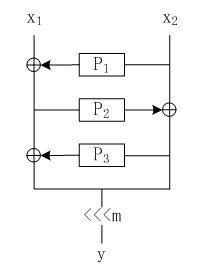
\includegraphics[scale=0.8]{zuc_sbox_p}
	\caption{Feistel network for S-box construction}
	\label{fig:zuc-sbox-p}
\end{figure}

The main idea behind the linear transformation in ZUC is high suitability for
software and hardware implementations and good diffusion properties. Therefore,
the transformation was defined using the quotient ring $GF(2)[x]/(x^{32}+1)$. A 32-bit word 
$a = a_{31} \, a_{30} \, \hdots \, a_0$ matches
an element $a(x)$ according to the bijection $\varphi$ from binary field
extension $GF(2^{32})$ to quotient ring $GF(2)[x]/(x^{32}+1)$ as follows:
\begin{equation}
\label{eqn:zuc-word-repr}
a =  a_{31} \, a_{30} \, \hdots \, a_0 \rightarrow a(x) =
\sum\limits_{i=0}^{31} a_i \, x^i \enspace.
\end{equation}

So the elements of linear transformation are represented by polynomials over
the quotient ring. Two polynomials define linear transformations used in ZUC: 
\begin{equation}
    \begin{array}{ll}
        L_1(x) = x^{24} + x^{18} + x^{10} + x^{2} + 1 \enspace, \\
        L_2(x) = x^{30} + x^{22} + x^{14} + x^{8} + 1 \enspace.
    \end{array}
\end{equation}

A transformation is performed by multiplying the input polynomial by $L_1$ or
$L_2$ . Such
transformations may be implemented by using cyclic shift and XOR operations
which are highly efficient both in software and hardware. ZUC developers also
noticed that the matrix representation of $L_1(x)$ and $L_2(x)$ over $GF(2)$
happen to be transpose matrices of each other.

\subsection{Initialization}
\label{sec:zuc-init}

Cipher key and initialization vector are split into bytes and combined with
15-bit constants defined in ZUC specification in order to load the key material
into LFSR stages which are 31 bits long. Each 15-bit constant substring is an
m-sequence generated by a primitive polynomial of degree 4 over the binary
field $GF(2)$~\cite{zuc:forum}. Initialization is done by clocking the cipher for 32 ticks. During
initialization the FSM output word $W$ is consumed by the LFSR update. Since
stages of LFSR are 31 bits long, the least significant bit of $W$ is removed by
right shift. If the resulting feedback value is 0, it is replaced by 
$p = 2^{31} - 1$ as zero stage is not allowed in $GF(2^{31}-1)$. 

\subsection{Keystream generation}
\label{sec:zuc-key-gen}

Keystream mode is similar to initialization, but the LFSR does not receive any
input. The output $W$ of non-linear function is XORed with $X_3$ (word extracted
on bit reorganization layer) producing keystream word $Z$. The very first word
produced by FSM after initialization is discarded. According to ZUC
specification the maximum length of keystream generated from a single key is
$65504$ bits (or $8188$ bytes). Such limitation is enforced by the LTE Service Data
Unit (SDU) size~\cite{zuc:dacas-page}.

\section{Implication of the finite state machine}
Analysis of the FSM revealed a drawback in linear transformations $L_1$ and
$L_2$. Given a symmetric input word (that is its lower 16 bits are equal to higher 16 bits)
the output of the transformation is also a symmetric word, thereby the power of
outputs set is reduced to $2^{16}$:
\begin{equation}
    \begin{array}{ll}
        L_1(\text{0x34BC34BC}) = \text{0x785A785A} ; \\
        L_2(\text{0xABCDABCD}) = \text{0x50C950C9} \enspace.
    \end{array}
\end{equation}

Equality in lower and higher half-words means that if the polynomial has a
coefficient $x^a$, than it also has a coefficient $x^{a + 16}$. Such behaviour of the linear
transformation can now be explained using polynomial arithmetic in quotient
ring. Consider an input polynomial of the form $x^a + x^{a+16}$ for
transformation $L_1$. Any
polynomial satisfying the described condition of symmetry may be chosen here
but for the sake of clarity only two coefficients are considered. The
transformation applies as follows:
\begin{equation}
    \label{eqn:zuc-symmetry}
	\begin{array}{ll}
        L_1(x^a + x^{a+16}) = (x^a + x^a x^16) \cdot (x^{24} + x^{18} + x^{10} + x^2 + 1) = \\
        = x^a \cdot (x^{24} + x^{18} + x^{10} + x^2 + 1) + x^{16} \cdot (x^{24} + x^{18} +x^{10} + x^2 +1) = \\
        = x^a \cdot (x^{24} + x^{18} + x^{10} + x^2 + 1 + \\
        + x^{24+16} + x^{18+16} + x^{10+16} + x^{2+16} + x^{16}) = \\
        = x^a \cdot (x^{24} + x^{22} + x^{14} + x^{8} + 1 + x^{40} + x^{34} + x^{26} + x^{18} + x^{16}) = \\
        = x^a \cdot (x^{26} + x^{24} + x^{16} + x^{10} + x^{8} + 1) \enspace .
	\end{array}
\end{equation}

So applying the linear transformation to any polynomial results to
multiplication of $x^a$ by 
$L_1 \cdot x^{16} + L_1 = x^{26} + x^{24} + x^{16} + x^{10} + x^{8} + 1$. 
This polynomial is symmetric as clearly seen from its
binary representation: 
$x^{26} + x^{24} + x^{16} + x^{10} + x^{8} + 1 = \text{0000 0101 0000 0001 0000 0101 0000 0001}$.

In fact the result of operation $L_1 \cdot x^a + L_1$ will always be symmetric in the chosen
quotient ring not depending on $L_1$ or $x^a$. Such behaviour is easy to explain
considering operations with binary representation of the polynomial.
Multiplication by $x^{16}$ in the quotient ring means left cyclic shift by 16 bits
which exchanges halves of the word. Addition of polynomials in  the quotient
ring is just XORing their binary representation. It is now clear from
figure~\ref{fig:zuc-symmetry}
that such transformation will always lead to symmetric output since left and
right parts of the word are XORed with each other. Following sections will
consider the influence of such property on the cipher security. 
\begin{figure}[htbp]
	\centering
	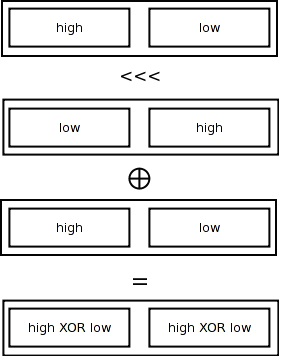
\includegraphics[scale=0.8]{zuc_symmetry}
	\caption{Linear transformation of symmetric input}
	\label{fig:zuc-symmetry}
\end{figure}

\section{Impact on cryptographic properties}

The S-boxes that follow linear transformation do not affect the symmetry of
words since they diffuse bits only within separate bytes. However the analysis
showed that there are still several obstacles on using the property for
cryptanalysis. The most effective transformations that corrupt symmetric words
inside the FSM are addition modulo $2^{32}$ and half-words exchanging.

\subsection{Symmetric words in bit reorganization layer}

With the possibility to choose both the cipher key and the IV it is possible to
make the words in Bit Reorganization layer symmetric. The initialization state
shown in~\eqref{zuc:symmetric-init} leads to symmetry in word $X_0$ for 1 tick, word $X_1$
for 2 ticks, $X_2$ for 7 ticks and $X_3$ for 12 ticks. The highlighted bytes indicate
that they may obtain any value and do not affect the symmetry in bit
reorganization layer words. Yet only the first output word of FSM is symmetric
because of the half-word exchanging, so registers are initialized by confused
values after the first tick. 
\begin{equation}
    \label{zuc:symmetric-init}
    \begin{array}{ll}
        s_{15} & \text{4D47AC00}\\
        s_{14} & \text{00789A8F}\\
        s_{13} & \text{003C4D35}\\
        s_{12} & \text{005E26D7}\\
        s_{11} & \text{269AF15E}\\
        s_{10} & \text{136BC49A}\\
        s_{9}  & \text{78AF1313}\\
        s_{8}  & \text{624D78E2}\\
        s_{7}  & \text{0989AF6B}\\
        s_{6}  & \text{3C7135AF}\\
        s_{5}  & \text{57B5E226}\\
        s_{4}  & \text{1AD789C4}\\
        s_{3}  & \text{71135E4D}\\
        s_{2}  & \text{44E26B89}\\
        s_{1}  & \text{2F26BC00}\\
        s_{0}  & \text{35C4D700}
    \end{array}
\end{equation}

If addition modulo $2^{32}$ is replaced by XOR and half-word exchanging is excluded,
the finite state machine is filled with symmetric words. However, the cipher
still resists to propagation of the linear transformation drawback due to
injecting $X_0$ into FSM. Symmetry in $X_0$ is destroyed with the second tick because of
the LFSR feedback which updates $s_{15}$. The effect of such initialization on
generated keystream is analyzed further.

\subsection{Randomness of cipher states on initialization}

Several statistical properties of LFSR state and keystream are considered.
Cross correlation between LFSR states after key loading and after
initialization indicates if any non-random relations remain after the
initialization procedure. Likewise, the cross correlation between LFSR state
after initialization and the first $496$ bits of keystream show if the starting
keystream bits depend on the initial LFSR state. Correlation of random
sequences oscillates near $0.5$ value (shown on graphs with green line), so the
larger deviation of correlation peaks from value $0.5$, the higher dependency
between them. 

Serial correlation coefficient measures the dependency of bits in the sequence
itself and obviously should be close to zero. Entropy shows the information
density of the binary data (maximum possible entropy in this case is 1 bit of
information per 1 bit of data).  Expected value (or arithmetic mean) is the
result of summing all the bits and dividing by the length of data. The value
should converge to $0.5$ in case of random data~\cite{Walker:ent}.

\subsection{LFSR state after initialization}

Results of statistical testing with corresponding values of keys and IVs are
presented in tables~\ref{tbl:lfsr-k0iv0}~--~\ref{tbl:lfsr-k1iv0}.

\begin{table}[htbp]
    \centering
    \caption{Statistical properties of LFSR state after initialization}
    \label{tbl:lfsr-k0iv0}
    \begin{tabular}{|l|l|} \hline
        Key     & all bytes equal 0x00  \\ \hline
        IV      & all bytes equal 0x00  \\ \hline 
        Entropy & 0.999295 per bit      \\ \hline 
        Arithmetic mean & 0.4844 \\ \hline 
        Serial correlation coefficient          & -0.047898 \\ \hline 
        Max cross correlation peak deviation    & 0.0678    \\ \hline
        Min cross correlation peak deviation    & 0.2081    \\ \hline
    \end{tabular}
\end{table}

Cross correlation tests indicate noticeable deviations from random values, so
it is possible to distinguish keys and IVs with long series of zeroes from
other random initialization values (figure~\ref{fig:lfsr-k0iv0}). However, the corresponding
keystream shows better results~\ref{tbl:keystream-k0iv0} and random cross
correlation~\ref{fig:keystream-k0iv0}.

The correlation deviation is observed again~\ref{fig:lfsr-k1iv1} for a different non-random
key and IV~\ref{tbl:lfsr-k1iv1}. But the corresponding keystream yet shows to be random.

In the testing sample on figure~\ref{tbl:lfsr-symmetric} the key and IV were chosen to
generate symmetric words in Bit Reorganization layer. No correlation deviations
or non-randomness signs have been found which indicates that the disadvantage
of linear transformations is annihilated by the cipher structure.

\begin{table}[htbp]
    \centering
    \caption{Statistical properties of first 496 keystream bits}
    \label{tbl:keystream-k0iv0}
    \begin{tabular}{|l|l|} \hline
        Key     & all bytes equal 0x00  \\ \hline
        IV      & all bytes equal 0x00  \\ \hline
        Entropy & 0.999840 per bit      \\ \hline
        Arithmetic mean & 0.4926        \\ \hline
        Serial correlation coefficient          & 0.025578  \\ \hline
        Max cross correlation peak deviation    & 0.0616    \\ \hline
        Min cross correlation peak deviation    & 0.0596    \\ \hline
    \end{tabular}
\end{table}

\begin{figure}[htbp]
	\centering
	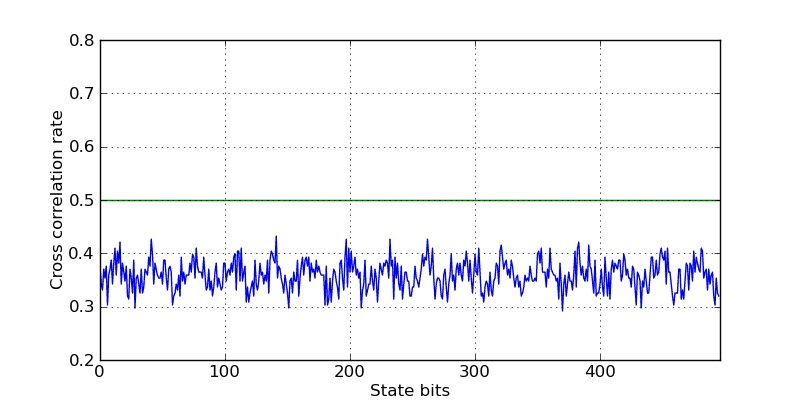
\includegraphics[scale=0.8]{zuc-lfsr-k0iv0}
	\caption{Cross correlation between LFSR initial state and after
    initialization (zero key, zero IV)}
	\label{fig:lfsr-k0iv0}
\end{figure}

\begin{figure}[htbp]
	\centering
	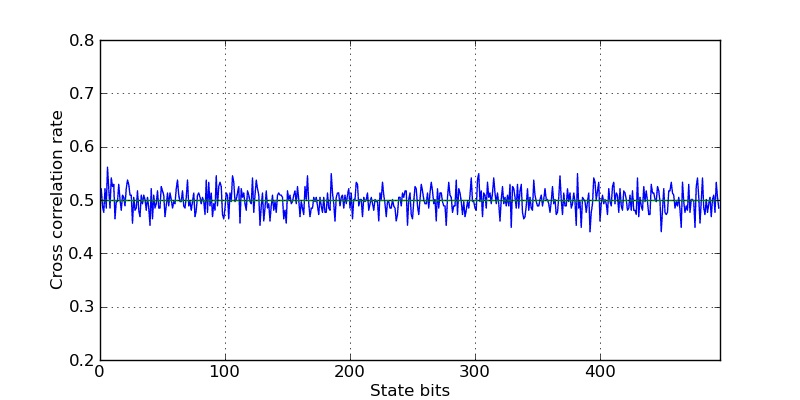
\includegraphics[scale=0.8]{zuc-lfsr-keystream}
	\caption{Cross correlation between LFSR state and keystream bits}
	\label{fig:keystream-k0iv0}
\end{figure}

\begin{table}[htbp]
    \centering
    \caption{Statistical properties LFSR state after initialization}
    \label{tbl:lfsr-k1iv1}
    \begin{tabular}{|l|l|} \hline
        Key & all bytes equal 0xFF \\ \hline
        IV & all bytes equal 0xFF \\ \hline
        Entropy & 0.991353 per bit \\ \hline
        Arithmetic mean & 0.4453 \\ \hline
        Serial correlation coefficient & 0.019521 \\ \hline
        Max cross correlation peak deviation & 0.1387 \\ \hline
        Min cross correlation peak deviation & 0.0509 \\ \hline
    \end{tabular}
\end{table}

\begin{figure}[htbp]
	\centering
	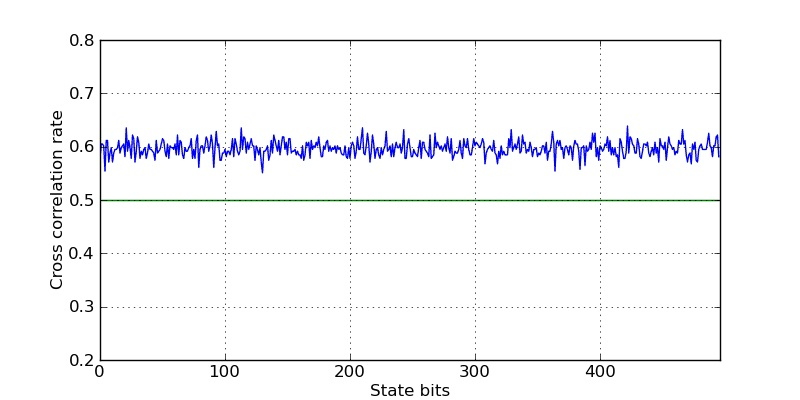
\includegraphics[scale=0.8]{zuc-lfsr-k1iv1}
	\caption{Cross correlation between LFSR initial state and after
    initialization (all key and IV bits equal 1)}
	\label{fig:lfsr-k1iv1}
\end{figure}

\begin{table}[htbp]
    \centering
    \caption{Statistical properties of LFSR state after initialization}
    \label{tbl:lfsr-symmetric}
    \begin{tabular}{|l|l|} \hline
        Key & generates symmetric words in BR \\ \hline
        IV & generates symmetric words in BR \\ \hline
        Entropy & 0.999725 per bit \\ \hline
        Arithmetic mean & 0.5098 \\ \hline
        Serial correlation coefficient & 0.007434 \\ \hline
    \end{tabular}
\end{table}

Further testing showed the corresponding keystream is random as well. All
tested random keys and IVs also resulted to good randomness of LFSR state and
generated keystream.  

If the key equals 0xFF and IV equals 0x0, the correlation
graphic shows normal deviation~\ref{tbl:lfsr-k1iv0} but periodic oscillation is
observed~\ref{fig:lfsr-k1iv0}.

\begin{table}[htbp]
    \centering
    \caption{Statistical properties of LFSR state after initialization}
    \label{tbl:lfsr-k1iv0}
    \begin{tabular}{|l|l|} \hline
        Key & all bytes equal 0xFF \\ \hline
        IV & all bytes equal 0x00 \\ \hline
        Max cross correlation peak deviation & 0.0603 \\ \hline
        Min cross correlation peak deviation & 0.0737 \\ \hline
    \end{tabular}
\end{table}

\begin{figure}[htbp]
	\centering
	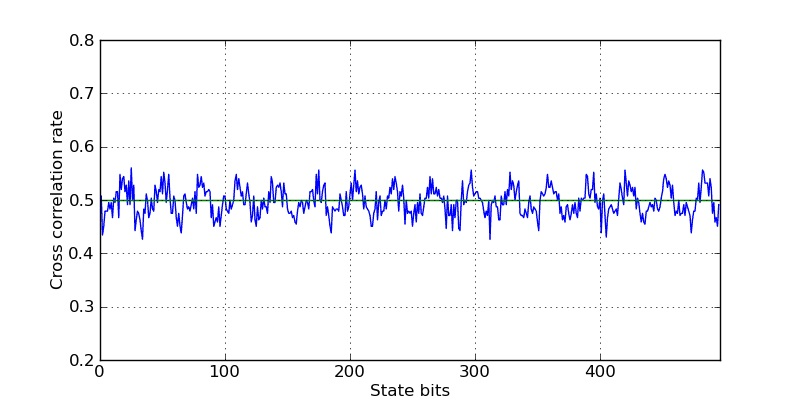
\includegraphics[scale=0.8]{zuc-lfsr-k1iv0}
	\caption{Cross correlation between LFSR initial state and after
    initialization (key bits equal 1, zero IV)}
	\label{fig:lfsr-k1iv0}
\end{figure}

Even though entropy, arithmetic mean and serial correlation tests show good
results, cross correlation testing of LFSR shows that it is possible to
distinguish some weak keys analysing the LFSR state after initialization
procedure. Non-random keys lead to bad randomization of LFSR state, but do not
noticeably influence generated keystreams. The property of the linear
transformations could not be used for an attack since the cipher structure
diffuses bits and destroys symmetry in output words within 2 ticks at worst.

No evidence of non-randomness in keystream bits has been found, but the testing
samples were too small for gathering enough statistics. Further the severe
randomness testing of ZUC keystream is performed using the set of tests
provided by NIST Statistical Test Suite~\cite{nist-sts}.

\subsection{Keystream randomness}

The cipher keystream has been analysed using test for randomness provided by
NIST. In order to get correct statistical results one needs to provide at least
55 data samples and each sample should be at least 1000000 bits long. According
to ZUC specification, the maximum length of keystream generated on a single key
is 65504 bits, so there is lack of data for performing all 15 tests from NIST
STS. Random Excursions and Random Excursions Variant tests are impossible to
perform with the specified amount of keystream data and therefore have been
excluded from evaluation. These tests actually represent 26 tests with
different parameters so the total amount of executed NIST STS tests is 163
instead of all 189.

Three keystream data sets have been tested for randomness: generated from
random keys, from non-random keys with long bit series, and from LFSR state that injects
symmetric words into BR layer. Results of testing the keystream randomness are
shown on figures~\ref{fig:zuc-stats-rand}~--~\ref{fig:zuc-stats-symmetric} and total
statistics are shown in table~\ref{tbl:zuc-stats}. Success rate shows how much
samples passed certain test (1 means all samples passed). The red line marks
minimum success rate in order to consider the sequence to be random.

\begin{table}[htbp]
    \centering
    \caption{Keystream randomness test summary}
    \label{tbl:zuc-stats}
    \begin{tabular}{|l|l|} \hline
        Type of initialization & Tests passed \\ \hline
        Random keys & 162/163 (99\%) \\ \hline
        Keys with long bit series & 162/163 (99\%) \\ \hline
        State that generates symmetric words in BR & 162/163 (99\%) \\ \hline
    \end{tabular}
\end{table}

\begin{figure}[htbp]
	\centering
	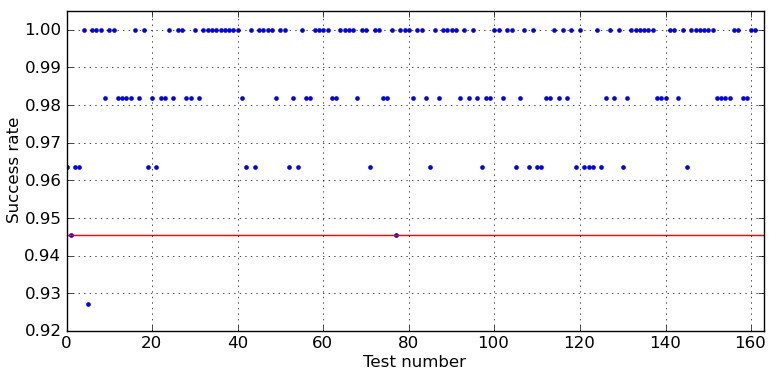
\includegraphics[scale=0.8]{zuc-stats-rand}
	\caption{Statistical testing results for random keys}
	\label{fig:zuc-stats-rand}
\end{figure}


\begin{figure}[htbp]
	\centering
	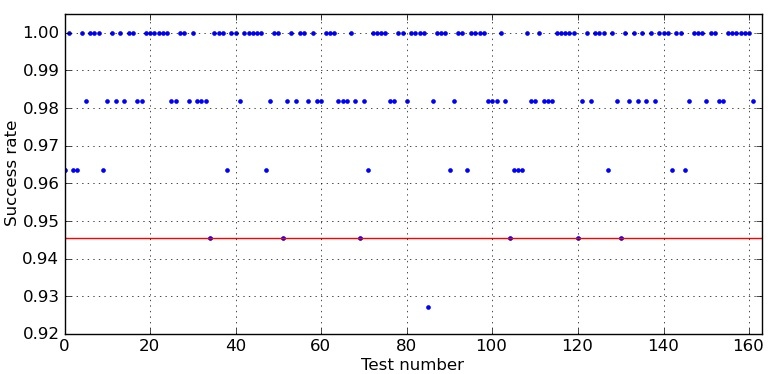
\includegraphics[scale=0.8]{zuc-stats-nonrand}
	\caption{Statistical testing results for non-random keys}
	\label{fig:zuc-stats-rand}
\end{figure}

\begin{figure}[htbp]
	\centering
	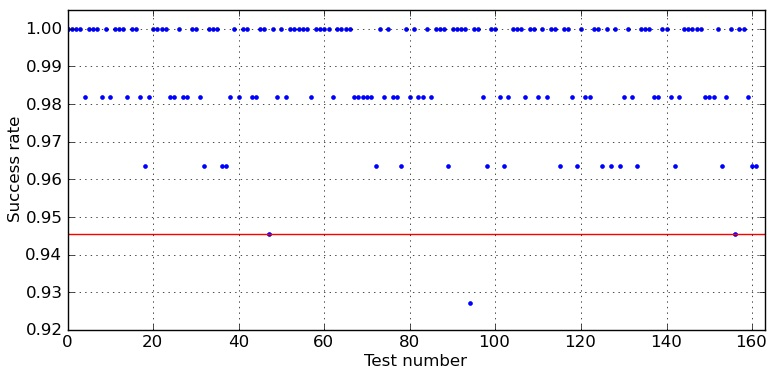
\includegraphics[scale=0.8]{zuc-stats-symmetric}
	\caption{Statistical testing results for BR symmetric words initialization}
	\label{fig:zuc-stats-symmetric}
\end{figure}
 
According to NIST STS in order for the keystream to be random 52 out of 55
samples should pass all statistical tests (in case of level of significance to
be 0.01). Keystream data set generated from random keys failed the Longest Run
test (51/55 samples passed). The other two keystream data sets failed the
Non-Overlapping Template Matching test for 1 of the 147 provided templates
(51/55 samples passed).

Even though the maximum keystream length used for encryption in LTE network on
single key is 65504 bits, the algorithm itself can produce any amount of data.
In order to make the testing more reliable two more data sets were produced to
satisfy Random Excursions and Random Excursions Variant test requirements. Both
keystreams generated from random and non-random keys successfully passed the
tests. Such results still indicate that the provided keystreams are
indistinguishable from truly random sequence and do not depend on the initial
key. Initializing the cipher with the state that injects symmetric words into
Bit Reorganization layer did not influence the keystream randomness.

\section{Results of cryptographic security analysis}

Detailed mathematical and statistical analysis of ZUC cipher revealed the
negligible defect in its linear transformation. Even though the structure of
ZUC effectively annihilates any consequences of the found property, such linear
transformations need improvement before being used for development of future
cryptographic algorithms in order to prevent possible weaknesses and losses of
entropy. As for ZUC, no evidence of weakness in the cipher caused by the linear
transformations in FSM could be found. The cipher has some set of weak keys
that cause bad randomization of LFSR state during initialization. Particularly
all non-random keys with long series of zeroes and ones result to non-random
state after initialization. However, such initialization states did not affect
the randomness of generated keystream.
